%Tech Science Press
%=================================================================
\documentclass[journal,article,submit,moreauthors,pdftex]{Definitions/tsp} 
%%%%Update on 30 November 2023%%%
\usepackage[normalem]{ulem} % For using the command \uuline{} in the \abstract 
\usepackage{amsfonts} % Use for some special math mark
%%\usepackage{pxfonts} % Use for some special math mark 
%\usepackage{wasysym} % Use for some special mark
%\usepackage{subfigure} % For some paper the use \subfigure
\usepackage{mathcomp} % For permille mark
\usepackage{CJKutf8} % For Chinese font
\usepackage{pifont} % For some special mark 
\usepackage{bm} % Forr math enviroment bold format
\usepackage{bbm} % For some math fancy characters
\graphicspath{{./Definitions/}} % Use for import path the figures paper used

\makeatletter
\def\T@n@@nc@d@ngM@cr@M@d{}
\def\LY@n@@nc@d@ngM@cr@M@d{}
\makeatother

\let\orignewcommand\newcommand  % Store the original \newcommand
\let\newcommand\providecommand  % Make \newcommand behave like \providecommand
\usepackage{verse}
\let\newcommand\orignewcommand  % Use the original `\newcommand` in future
\makeatletter
\renewcommand*{\theHpoemline}{\arabic{verse@envctr}.\arabic{poemline}} % Use the original definition from verse.sty
\makeatother

% Define a matrix envrioment
\newsavebox\foobox
\newcommand{\slantbox}[2][.2]{\mbox{%
        \sbox{\foobox}{#2}%
        \hskip\wd\foobox
        \pdfsave
        \pdfsetmatrix{1 0 #1 1}%
        \llap{\usebox{\foobox}}%
        \pdfrestore
}}

%\setlength{\fboxsep}{0cm}

% Define triangledown mark
\let\oldblacktriangledown\blacktriangledown

% Define \dagger using unicode
\renewcommand{\dagger}{\mathchar"2279}
\renewcommand{\ddagger}{\mathchar"227A}

% Define italic In, Max
\newcommand{\mmathit}[1]{
  \ifthenelse{\equal{#1}{\ln}}{\mathit{ln}}{
    \ifthenelse{\equal{#1}{\max}}{\mathit{max}}{\mathit{#1}}
  }
}
\makeatother
\robustify{\footnote}

\DeclareUnicodeCharacter{1E45}{\.{n}}
\DeclareUnicodeCharacter{1E41}{\.{m}}
\DeclareUnicodeCharacter{2003}{\quad}
%\DeclareUnicodeCharacter{0177}{\^{y}}
%\DeclareUnicodeCharacter{101}{\={a}}
\DeclareUnicodeCharacter{2009}{\thinspace}
\DeclareUnicodeCharacter{2002}{\enspace{}}
\DeclareUnicodeCharacter{2005}{\thinspace}
\DeclareUnicodeCharacter{0263}{\textipa{G}}
%\DeclareUnicodeCharacter{117}{\.{e}}
\DeclareUnicodeCharacter{A0}{~}
\DeclareUnicodeCharacter{2460}{\textcircled{\scriptsize{1}}}
\DeclareUnicodeCharacter{2461}{\textcircled{\scriptsize{2}}}
\DeclareUnicodeCharacter{2462}{\textcircled{\scriptsize{3}}}
\DeclareUnicodeCharacter{2463}{\textcircled{\scriptsize{4}}}
\DeclareUnicodeCharacter{2464}{\textcircled{\scriptsize{5}}}
\DeclareUnicodeCharacter{2465}{\textcircled{\scriptsize{6}}}
\DeclareUnicodeCharacter{2466}{\textcircled{\scriptsize{7}}}
\DeclareUnicodeCharacter{2467}{\textcircled{\scriptsize{8}}}
\DeclareUnicodeCharacter{2468}{\textcircled{\scriptsize{9}}}
\DeclareUnicodeCharacter{2070}{\textsuperscript{0}}
\DeclareUnicodeCharacter{2074}{\textsuperscript{4}}
\DeclareUnicodeCharacter{2075}{\textsuperscript{5}}
\DeclareUnicodeCharacter{2076}{\textsuperscript{6}}
\DeclareUnicodeCharacter{2077}{\textsuperscript{7}}
\DeclareUnicodeCharacter{2078}{\textsuperscript{8}}
\DeclareUnicodeCharacter{2079}{\textsuperscript{9}}
\DeclareUnicodeCharacter{02C2}{<}
\DeclareUnicodeCharacter{2033}{\relax\ifmmode '' \else $''$\fi}
\DeclareUnicodeCharacter{2034}{\relax\ifmmode ''' \else $'''$\fi}
\DeclareUnicodeCharacter{2026}{\relax\ifmmode … \else $\ldots$\fi}
\DeclareUnicodeCharacter{0229}{\c{e}}
\DeclareUnicodeCharacter{016F}{\r{u}}
%\DeclareUnicodeCharacter{0218}{\cb{S}}
%\DeclareUnicodeCharacter{0219}{\cb{s}}
%\DeclareUnicodeCharacter{021B}{\cb{t}}
\DeclareUnicodeCharacter{127}{\relax\ifmmode\rm\hbar\else $\rm\hbar$\fi}
\DeclareUnicodeCharacter{3AC}{\relax\ifmmode\acute{\alpha}\else $\acute{\alpha}$\fi}
\DeclareUnicodeCharacter{3AD}{\relax\ifmmode\acute{\varepsilon}\else $\acute{\varepsilon}$\fi}
\DeclareUnicodeCharacter{3AE}{\relax\ifmmode\acute{\eta}\else $\acute{\eta}$\fi}
\DeclareUnicodeCharacter{3AF}{\relax\ifmmode\acute{\iota}\else $\acute{\iota}$\fi}
\DeclareUnicodeCharacter{3CC}{\relax\ifmmode\acute{o}\else $\acute{o}$\fi}
\DeclareUnicodeCharacter{3CD}{\relax\ifmmode\acute{\upsilon}\else $\acute{\upsilon}$\fi}
\DeclareUnicodeCharacter{3CE}{\relax\ifmmode\acute{\omega}\else $\acute{\omega}$\fi}
\DeclareUnicodeCharacter{391}{A}
\DeclareUnicodeCharacter{392}{B}
\DeclareUnicodeCharacter{395}{E}
\DeclareUnicodeCharacter{396}{Z}
\DeclareUnicodeCharacter{397}{H}
\DeclareUnicodeCharacter{399}{I}
\DeclareUnicodeCharacter{39A}{K}
\DeclareUnicodeCharacter{39C}{M}
\DeclareUnicodeCharacter{39D}{N}
\DeclareUnicodeCharacter{39F}{O}
\DeclareUnicodeCharacter{3A1}{P}
\DeclareUnicodeCharacter{3A4}{T}
\DeclareUnicodeCharacter{3A7}{X}

\DeclareUnicodeCharacter{27E6}{\relax\ifmmode \llbracket \else $\llbracket$\fi}
\DeclareUnicodeCharacter{27E7}{\relax\ifmmode \rrbracket \else $\rrbracket$\fi}
\DeclareUnicodeCharacter{00B5}{\relax\ifmmode \mu{} \else $\mu$\fi}
\DeclareUnicodeCharacter{1D434}{\relax\ifmmode A \else $A$\fi}
\DeclareUnicodeCharacter{1D435}{\relax\ifmmode B \else $B$\fi}
\DeclareUnicodeCharacter{1D436}{\relax\ifmmode C \else $C$\fi}
\DeclareUnicodeCharacter{1D437}{\relax\ifmmode D \else $D$\fi}
\DeclareUnicodeCharacter{1D438}{\relax\ifmmode E \else $E$\fi}
\DeclareUnicodeCharacter{1D439}{\relax\ifmmode F \else $F$\fi}
\DeclareUnicodeCharacter{1D43A}{\relax\ifmmode G \else $G$\fi}
\DeclareUnicodeCharacter{1D43B}{\relax\ifmmode H \else $H$\fi}
\DeclareUnicodeCharacter{1D43C}{\relax\ifmmode I \else $I$\fi}
\DeclareUnicodeCharacter{1D43D}{\relax\ifmmode J \else $J$\fi}
\DeclareUnicodeCharacter{1D43E}{\relax\ifmmode K \else $K$\fi}
\DeclareUnicodeCharacter{1D43F}{\relax\ifmmode L \else $L$\fi}
\DeclareUnicodeCharacter{1D440}{\relax\ifmmode M \else $M$\fi}
\DeclareUnicodeCharacter{1D441}{\relax\ifmmode N \else $N$\fi}
\DeclareUnicodeCharacter{1D442}{\relax\ifmmode O \else $O$\fi}
\DeclareUnicodeCharacter{1D443}{\relax\ifmmode P \else $P$\fi}
\DeclareUnicodeCharacter{1D444}{\relax\ifmmode Q \else $Q$\fi}
\DeclareUnicodeCharacter{1D445}{\relax\ifmmode R \else $R$\fi}
\DeclareUnicodeCharacter{1D446}{\relax\ifmmode S \else $S$\fi}
\DeclareUnicodeCharacter{1D447}{\relax\ifmmode T \else $T$\fi}
\DeclareUnicodeCharacter{1D448}{\relax\ifmmode U \else $U$\fi}
\DeclareUnicodeCharacter{1D449}{\relax\ifmmode V \else $V$\fi}
\DeclareUnicodeCharacter{1D44A}{\relax\ifmmode W \else $W$\fi}
\DeclareUnicodeCharacter{1D44B}{\relax\ifmmode X \else $X$\fi}
\DeclareUnicodeCharacter{1D44C}{\relax\ifmmode Y \else $Y$\fi}
\DeclareUnicodeCharacter{1D44D}{\relax\ifmmode Z \else $Z$\fi}
\DeclareUnicodeCharacter{1D44E}{\relax\ifmmode a \else $a$\fi}
\DeclareUnicodeCharacter{1D44F}{\relax\ifmmode b \else $b$\fi}
\DeclareUnicodeCharacter{1D450}{\relax\ifmmode c \else $c$\fi}
\DeclareUnicodeCharacter{1D451}{\relax\ifmmode d \else $d$\fi}
\DeclareUnicodeCharacter{1D452}{\relax\ifmmode e \else $e$\fi}
\DeclareUnicodeCharacter{1D453}{\relax\ifmmode f \else $f$\fi}
\DeclareUnicodeCharacter{1D454}{\relax\ifmmode g \else $g$\fi}
\DeclareUnicodeCharacter{1D456}{\relax\ifmmode i \else $i$\fi}
\DeclareUnicodeCharacter{1D457}{\relax\ifmmode j \else $j$\fi}
\DeclareUnicodeCharacter{1D458}{\relax\ifmmode k \else $k$\fi}
\DeclareUnicodeCharacter{1D459}{\relax\ifmmode l \else $l$\fi}
\DeclareUnicodeCharacter{1D45A}{\relax\ifmmode m \else $m$\fi}
\DeclareUnicodeCharacter{1D45B}{\relax\ifmmode n \else $n$\fi}
\DeclareUnicodeCharacter{1D45C}{\relax\ifmmode o \else $o$\fi}
\DeclareUnicodeCharacter{1D45D}{\relax\ifmmode p \else $p$\fi}
\DeclareUnicodeCharacter{1D45E}{\relax\ifmmode q \else $q$\fi}
\DeclareUnicodeCharacter{1D45F}{\relax\ifmmode r \else $r$\fi}
\DeclareUnicodeCharacter{1D460}{\relax\ifmmode s \else $s$\fi}
\DeclareUnicodeCharacter{1D461}{\relax\ifmmode t \else $t$\fi}
\DeclareUnicodeCharacter{1D462}{\relax\ifmmode u \else $u$\fi}
\DeclareUnicodeCharacter{1D463}{\relax\ifmmode v \else $v$\fi}
\DeclareUnicodeCharacter{1D464}{\relax\ifmmode w \else $w$\fi}
\DeclareUnicodeCharacter{1D465}{\relax\ifmmode x \else $x$\fi}
\DeclareUnicodeCharacter{1D466}{\relax\ifmmode y \else $y$\fi}
\DeclareUnicodeCharacter{1D467}{\relax\ifmmode z \else $z$\fi}

\DeclareUnicodeCharacter{1E67}{\.{\v s}}
\DeclareUnicodeCharacter{1E11}{\relax\ifmmode \c{d} \else $\c{d}$\fi}
\DeclareUnicodeCharacter{1ECB}{\relax\ifmmode \d{i} \else $\d{i}$\fi}
\DeclareUnicodeCharacter{1D8D}{\relax\ifmmode \textlhookx \else $\textlhookx$\fi}
\DeclareUnicodeCharacter{104}{\relax\ifmmode \k{A} \else $\k{A}$\fi}
\DeclareUnicodeCharacter{211E}{\relax\ifmmode \textrecipe \else $\textrecipe$\fi}
\DeclareUnicodeCharacter{29D}{\relax\ifmmode \textctj \else $\textctj$\fi}

\DeclareUnicodeCharacter{1E2E}{\'{\"I}}
\DeclareUnicodeCharacter{23F}{\textrts}

\DeclareUnicodeCharacter{2C73}{\varw}

\DeclareUnicodeCharacter{2127}{\mho}

\DeclareUnicodeCharacter{28C}{\textturnv}
\DeclareUnicodeCharacter{252}{\textturnscripta}
\DeclareUnicodeCharacter{259}{\schwa}
\DeclareUnicodeCharacter{25B}{\m{e}}
\DeclareUnicodeCharacter{266}{\m{h}}
\DeclareUnicodeCharacter{127}{\B{h}}
\DeclareUnicodeCharacter{27E}{\textfishhookr}
\DeclareUnicodeCharacter{281}{\textinvscr}



% Article metadata commands
\continuouspages{}
\firstpage{1} 
\makeatletter 
\setcounter{page}{\@firstpage} 
\makeatother
\pubvolume{0}
\issuenum{0}
\elocationid{0}
\articlenumber{0}
\pubyear{2026}
\copyrightyear{2026}
\datereceived{Day Month Year}
\dateaccepted{Day Month Year}
\dateonlinefirst{}
\datepublished{Day Month Year}
\setlength{\abovedisplayskip}{4pt}
\setlength{\belowdisplayskip}{4pt}

% Supplementary packages (only non-duplicates not already loaded by tsp.cls)
\usepackage{threeparttable}
\usepackage{algorithm}
\usepackage{algpseudocode}
\usepackage{makecell}
\usepackage{adjustbox}

% Neutralize blank page ejection in article maketitle
\makeatletter
\let\orig@maketitle\maketitle
\def\maketitle{\let\newpage\relax\orig@maketitle}
\makeatother

% Full title of the paper
\Title{PneuSSLNet: A Unified Self-Supervised Learning Framework for Pneumonia Classification from Chest X-Ray Images}

\Author{S. M. Mubasshir Al Kasshaf\textsuperscript{1}, Md. Faruk Hosen\textsuperscript{1}, S M Hasan Mahmud\textsuperscript{2}, Marzia Diya Khan\textsuperscript{1}, Kah Ong Michael Goh\textsuperscript{3,*}, and Md Imam Ahasan\textsuperscript{4}}

% Authors for metadata in PDF
\AuthorNames{S. M. Mubasshir Al Kasshaf, Md. Faruk Hosen, S M Hasan Mahmud, Marzia Diya Khan, Kah Ong Michael Goh, and Md Imam Ahasan}

% Affiliations / Addresses
\address{%
\textsuperscript{1}Department of Computer Science and Engineering, Begum Rokeya University, Rangpur 5400, Bangladesh\\
\textsuperscript{2}Department of Software Engineering, Daffodil International University, Savar, Dhaka 1216, Bangladesh\\
\textsuperscript{3}Center for Image and Vision Computing, COE for Artificial Intelligence, Faculty of Information Science \& Technology (FIST), Multimedia University, Melaka 75450, Malaysia\\
\textsuperscript{4}College of Computer Science, Chongqing University, Chongqing 400044, China
}%

% Contact information of the corresponding author
\corres{Correspondence: Kah Ong Michael Goh. Email: michael.goh@mmu.edu.my}

% Abstract
\abstract{Pneumonia is a leading cause of pediatric morbidity and mortality worldwide, where timely and accurate chest radiograph (CXR) interpretation is essential for clinical management. However, supervised deep learning models require massive expert-annotated cohorts, which are prohibitively costly, time-consuming, and prone to inter-observer variability. Self-supervised learning (SSL) provides an attractive paradigm by learning invariant visual representations from unlabeled radiographs prior to task-specific transfer. In this study, we propose \textbf{PneuSSLNet}, a unified, multi-paradigm self-supervised learning and evaluation framework for pediatric pneumonia diagnosis from chest radiographs. PneuSSLNet establishes a controlled, head-to-head benchmark across four foundational SSL paradigms---SimCLR (contrastive with negative pairs), MoCo (contrastive with memory queue and momentum encoder), BYOL (negative-free bootstrap prediction), and DINO (self-distillation with multi-crop local-global views)---interfaced with two complementary architectures: ResNet-50 (23.5M parameters) and EfficientNet-B0 (4.0M parameters). To resolve test-set leakage present in previous studies, all representations were transferred via a two-stage progressive downstream adaptation protocol (frozen linear head warmup followed by differential backbone unfreezing with cosine learning-rate scheduling) trained on a verified stratified partition (70\% train, 15\% validation, and an untouched 15\% locked test set). Under this controlled protocol, \textbf{DINO combined with EfficientNet-B0} achieved the highest overall diagnostic performance on the held-out test cohort ($N = 879$), reaching an accuracy of \textbf{97.38\%}, precision of \textbf{98.89\%}, recall (sensitivity) of \textbf{97.50\%}, F1-score of \textbf{98.19\%}, and an AUROC of \textbf{99.34\%}, while requiring 83\% fewer parameters than ResNet-50. Systematic label-efficiency sweeps demonstrated that SSL models maintain clinical diagnostic viability ($>94\%$ accuracy) even when fine-tuned with as little as 10\% labeled data, substantially outperforming supervised models trained from scratch. Furthermore, to evaluate out-of-distribution domain generalization, the champion model was validated on the external RSNA Pneumonia Detection cohort ($N = 26,684$ DICOM radiographs from independent healthcare centers), achieving a zero-shot cross-center AUROC of \textbf{93.45\%} and sensitivity of \textbf{91.35\%} in differentiating pneumonia from normal cases, with a negative predictive value of \textbf{95.36\%}. Clinically driven Explainable AI (Grad-CAM) with edge-randomization sanity checks confirmed biologically plausible attention localized to focal pulmonary infiltrates and perihilar opacities. PneuSSLNet provides an empirically rigorous, reproducible, and lightweight framework for label-efficient chest radiograph analysis in resource-constrained healthcare environments.}

\keyword{Pneumonia Classification, Self-Supervised Learning, Chest Radiography, Representation Learning, SimCLR, MoCo, BYOL, DINO, EfficientNet, Explainable AI, External Clinical Validation}

\begin{document}

\section{Introduction} \label{sect:s1}

Pneumonia remains one of the deadliest infectious diseases globally, accounting for over 740,000 deaths annually among children under five years of age, predominantly in low- and middle-income countries \cite{WHO2022,Kermany18}. Chest radiography (CXR) serves as the primary first-line imaging modality for confirming pulmonary consolidations, infiltrates, and bronchopneumonia due to its widespread accessibility, low radiation dosage, and rapid acquisition \cite{Rajpurkar17}. Nevertheless, clinical radiograph interpretation in resource-constrained clinical settings is severely constrained by an acute shortage of certified thoracic radiologists, high daily caseloads, and considerable inter- and intra-observer diagnostic discordance, especially in early or atypical pediatric presentations \cite{Sowrirajan21,Huang23}.

To mitigate these clinical burdens, automated computer-aided diagnostic systems powered by deep convolutional neural networks (CNNs) have been widely developed \cite{ElAsnaoui21,Kundu21}. Prominent milestones such as Kermany et al. \cite{Kermany18} and CheXNet \cite{Rajpurkar17} established the technical viability of deep networks for radiograph interpretation. Subsequent studies explored diverse enhancements, including model ensembles \cite{Kundu21,Mabrouk22}, neural architecture search (NAS) \cite{Gupta22}, attention mechanisms \cite{Singh23,Asswin23}, weakly supervised lesion localization \cite{Guo23}, and Vision Transformers (ViTs) \cite{Singh24,Ha23}. However, conventional supervised deep learning remains inherently vulnerable to the \emph{annotation bottleneck}: learning discriminative features requires extensive, high-quality, pixel- or image-level manual annotations by experienced radiologists. In clinical medicine, acquiring such annotations is prohibitively expensive, time-intensive, privacy-restricted, and subject to diagnostic subjectivity \cite{Huang23,Azizi21}.

Self-Supervised Learning (SSL) has emerged as a transformative paradigm that directly addresses this annotation bottleneck by learning generalized visual representations from unlabeled radiographs without requiring manual diagnostic ground truth \cite{Chen20,He20,Tiu22}. By formulating pretext tasks grounded in visual invariance---such as maximizing mutual information across stochastic augmentations or predicting representations across online and momentum encoders---SSL enables deep networks to discover intrinsic anatomical features (e.g., rib structures, diaphragmatic contours, vascular markings, and parenchymal opacities) directly from raw imaging data \cite{Grill20,Caron21}. When subsequently transferred to downstream clinical classification, SSL-pretrained representations have shown marked improvements in label efficiency, out-of-distribution robustness, and transferability across chest radiograph benchmarks \cite{Sowrirajan21,Tiu22,Cho23}.

Despite these promising advances, existing literature on SSL in chest radiography exhibits three critical scientific and methodological shortcomings:
\begin{enumerate}
    \item \textbf{Absence of Controlled Multi-Paradigm Benchmarks:} Most prior studies examine an isolated SSL algorithm (predominantly SimCLR or MoCo) on a single backbone, confounding pretraining objective differences with architectural variations, conflicting data augmentations, and disparate downstream fine-tuning schedules \cite{Gazda21,Han21,SinghMLVICX24}. A systematic, head-to-head comparison across the three major self-supervised learning families---contrastive learning with explicit negative pairs (SimCLR, MoCo), non-contrastive bootstrap prediction (BYOL), and self-distillation (DINO)---under an identical data pipeline and compute envelope has not been established for pediatric pneumonia.
    \item \textbf{Widespread Validation Flaws and Test-Set Leakage:} As documented in recent methodological audits \cite{Bundele24}, many published medical imaging studies suffer from structural validation flaws, including minuscule validation cohorts (e.g., 16 images), in-loop hyperparameter and threshold tuning directly on the test cohort, and single-run evaluations devoid of variance or statistical significance reporting. Consequently, reported performance metrics often overestimate clinical generalization.
    \item \textbf{Lack of Rigorous External Clinical Validation:} The overwhelming majority of CXR pneumonia models are trained and tested on images acquired from a single medical center with homogenous acquisition hardware and demographics \cite{Kermany18,ElAsnaoui21}. Without zero-shot out-of-distribution (OOD) validation on multi-institutional, full-resolution hospital DICOM cohorts, model readiness for real-world clinical deployment remains unproven.
\end{enumerate}

To rigorously address these challenges, we propose \textbf{PneuSSLNet}, a unified, multi-paradigm self-supervised learning and evaluation framework for pediatric pneumonia diagnosis from chest radiographs. PneuSSLNet establishes a controlled, fair, and reproducible benchmark that systematically decouples representation learning from supervised classification across four established SSL paradigms (SimCLR, MoCo, BYOL, DINO) and two complementary convolutional backbones: ResNet-50 (a deep residual baseline with 23.5M parameters) \cite{He16} and EfficientNet-B0 (a compound-scaled lightweight architecture with 4.0M parameters) \cite{Tan19}. 

The principal scientific and clinical contributions of this work are summarized as follows:
\begin{itemize}
    \item \textbf{Unified Four-Method Multi-Paradigm Benchmark:} We design and implement a strictly standardized pretraining and evaluation suite that compares SimCLR, MoCo, BYOL, and DINO under identical stochastic transformation spaces, projection dimensions (512-hidden, 128-embedding), and batch geometries.
    \item \textbf{Leakage-Free Two-Stage Progressive Adaptation Protocol:} We introduce a two-stage downstream transfer mechanism consisting of Stage~1 linear head warmup with frozen feature extractors, followed by Stage~2 differential backbone unfreezing with cosine annealing. Crucially, a strict \emph{Test-Set Firewall} is enforced: all hyperparameters, checkpoint selections, and threshold calibrations occur strictly on a verified 15\% validation split, with the held-out test cohort ($N=879$) evaluated exactly once at study conclusion.
    \item \textbf{State-of-the-Art Diagnostic Performance with Green AI Efficiency:} We demonstrate that DINO coupled with EfficientNet-B0 establishes the highest overall diagnostic performance across all evaluated models, achieving an accuracy of \textbf{97.38\%}, F1-score of \textbf{98.19\%}, precision of \textbf{98.89\%}, and an AUROC of \textbf{99.34\%} on unseen internal test radiographs, outperforming ResNet-50 while requiring 83\% fewer parameters and 60\% less GPU memory.
    \item \textbf{Systematic Label-Efficiency Quantification:} We conduct extensive empirical sweeps across labeled training subsets (10\%, 25\%, 50\%, 75\%, 100\%), proving that SSL pretraining preserves diagnostic utility ($>94\%$ accuracy) even with minimal labeled supervision, providing substantial margins over supervised models trained from scratch.
    \item \textbf{Large-Scale Multi-Center External DICOM Validation:} We validate the champion model on the complete RSNA Pneumonia Detection Challenge cohort ($N=26,684$ DICOM radiographs), demonstrating a zero-shot OOD AUROC of \textbf{93.45\%} and sensitivity of \textbf{91.35\%} on pneumonia versus normal cases, accompanied by a negative predictive value of \textbf{95.36\%}.
    \item \textbf{Clinically Grounded Explainability and Sanity Verification:} We integrate Gradient-weighted Class Activation Mapping (Grad-CAM) to visualize pulmonary consolidation attention, accompanied by cascading weight randomization sanity checks confirming biological plausibility.
\end{itemize}

\section{Related Works} \label{sect:s2}

\subsection{Supervised Deep Learning for Chest Radiograph Analysis}
The application of convolutional neural networks to chest radiographs gained significant momentum following the public release of benchmark datasets such as ChestX-ray14 \cite{Wang17}, CheXpert \cite{Irvin19}, MIMIC-CXR \cite{Johnson19}, and the pediatric pneumonia cohort compiled by Kermany et al. \cite{Kermany18}. Kermany et al. utilized transfer learning with Inception-V3, achieving 92.8\% accuracy and 93.2\% recall. Subsequent studies explored diverse architectural variants: El Asnaoui et al. \cite{ElAsnaoui21} benchmarked classic architectures, reporting 96.61\% accuracy with ResNet-50, while Chouhan et al. \cite{Chouhan20} and Elshennawy and Ibrahim \cite{Elshennawy20} evaluated deep transfer learning pipelines.

To enhance classification stability, ensemble and multi-scale strategies were introduced. Kundu et al. \cite{Kundu21} proposed a weighted decision fusion ensemble combining GoogLeNet, ResNet-18, and DenseNet-121, reporting an accuracy of 98.81\% and an AUC of 98.35\%. Mabrouk et al. \cite{Mabrouk22} utilized an ensemble of DenseNet-169, MobileNet-V2, and ViT, achieving 93.91\% accuracy. Other researchers explored architecture optimization via neural architecture search (NAS); Gupta et al. \cite{Gupta22} developed LBT-PC-DARTS, achieving 97.00\% accuracy and 97.60\% AUC across 5-fold cross-validation. Attention-based models were also pursued: Islam et al. \cite{Singh23} proposed the Quaternion Channel-Spatial Attention (QCSA) network, achieving 94.53\% accuracy, while Asswin et al. \cite{Asswin23} incorporated channel attention into pediatric diagnosis. More recently, Vision Transformers were deployed: Singh et al. \cite{Singh24} implemented ViT and DeiT architectures, achieving 97.61\% accuracy, and Ha et al. \cite{Ha23} investigated self-attention mechanisms for radiographic feature extraction.

Despite these notable metrics, all aforementioned studies rely strictly on supervised pretraining or full supervision. As synthesized in Table~\ref{tab:related_works}, supervised paradigms remain critically vulnerable to label scarcity, annotation noise, and cross-scanner domain shifts.

\subsection{Self-Supervised Learning Paradigms in Medical Imaging}
Self-supervised learning has revolutionized visual representation learning by deriving supervisory signals directly from data structure \cite{Huang23}. Contemporary SSL methods can be grouped into three distinct paradigm families:
\begin{enumerate}
    \item \textbf{Contrastive Learning with Explicit Negatives:} SimCLR (Chen et al. \cite{Chen20}) optimizes the Normalized Temperature-scaled Cross-Entropy (NT-Xent) loss, maximizing agreement between differently augmented views of the same image while actively repelling negative samples within the mini-batch. MoCo (He et al. \cite{He20}) decouples dictionary size from mini-batch size by maintaining a dynamic memory queue of negative representations and updating a key encoder via an exponential moving average (EMA). Sowrirajan et al. \cite{Sowrirajan21} and Gazda et al. \cite{Gazda21} demonstrated that MoCo pretraining improves representation transferability on chest radiographs.
    \item \textbf{Negative-Free Bootstrap Learning:} BYOL (Grill et al. \cite{Grill20}) discards negative pairs entirely, training an online network to predict the representation of a target network updated via momentum. By incorporating an asymmetric predictor head, BYOL prevents representation collapse without contrastive repulsion. Han et al. \cite{Han21} combined contrastive and radiomic features to enhance interpretability under limited supervision.
    \item \textbf{Self-Distillation Paradigms:} DINO (Caron et al. \cite{Caron21}) formulates self-supervision as knowledge distillation without labels, where a student network predicts the output distribution of a momentum teacher network. By combining centering, temperature sharpening, and a multi-crop strategy (global views capturing semantic context and local crops capturing fine details), DINO learns rich spatial hierarchies. Shakouri et al. \cite{Shakouri23} applied DINO with Vision Transformers to chest radiographs, highlighting its localization capabilities.
\end{enumerate}

Broad medical imaging surveys by Huang et al. \cite{Huang23}, Tiu et al. \cite{Tiu22}, Azizi et al. \cite{Azizi21}, and Bundele et al. \cite{Bundele24} have demonstrated that self-supervised pretraining substantially improves downstream label efficiency and clinical robustness. However, existing CXR studies have primarily examined SSL in isolation without directly contrasting these foundational paradigms under a standardized, leak-free evaluation protocol. PneuSSLNet bridges this critical gap.

\begin{table*}[t]
\tablesize{\scriptsize}
\centering
\caption{Comprehensive summary of representative related works on deep-learning-based pneumonia classification from chest radiography.}
\label{tab:related_works}
\begin{threeparttable}
\begin{adjustbox}{max width=\textwidth}
\begin{tabular}{p{2.8cm} p{2.2cm} p{2.4cm} p{4.6cm} p{5.2cm}}
\toprule
\textbf{Study} & \textbf{Dataset(s)} & \textbf{Learning Paradigm} & \textbf{Core Methodology / Architecture} & \textbf{Reported Findings / Limitations} \\
\midrule
Kermany et al. \cite{Kermany18} & Kermany CXR & Supervised Transfer & Inception-V3 ImageNet pretraining & Acc: 92.8\%, Rec: 93.2\%; supervised benchmark. \\
El Asnaoui et al. \cite{ElAsnaoui21} & Kermany CXR & Supervised Transfer & ResNet-50, VGG-16, DenseNet-201 & Acc: 96.61\%, Prec: 98.49\%; single-center only. \\
Kundu et al. \cite{Kundu21} & Kermany + RSNA & Supervised Ensemble & GoogLeNet + ResNet-18 + DenseNet-121 & Acc: 98.81\%, AUC: 98.35\%; high compute cost. \\
Gupta et al. \cite{Gupta22} & Kermany CXR & Neural Arch Search & LBT-PC-DARTS gradient-based NAS & Acc: 97.00\%, AUC: 97.60\%; complex search space. \\
Singh et al. \cite{Singh23} & Kermany CXR & Supervised Attention & Quaternion CNN + Channel-Spatial Attention & Acc: 94.53\%, AUC: 89.00\%; specialized design. \\
Guo et al. \cite{Guo23} & Kermany + RAIG & Weakly Supervised & ResNet-34 + Class Activation Mapping & Acc: 98.29\%, AUC: 99.49\%; multi-center evaluation. \\
Singh et al. \cite{Singh24} & Kermany CXR & Vision Transformer & ViT / DeiT patch self-attention & Acc: 97.61\%, AUC: 96.60\%; high data requirements. \\
Sowrirajan et al. \cite{Sowrirajan21} & CheXpert & Self-Supervised & MoCo-v2 pretraining on CXR & Outperformed ImageNet initialization at low labels. \\
Gazda et al. \cite{Gazda21} & ChestX-ray14 & Self-Supervised & Fully self-supervised contrastive learning & Evaluated label efficiency; contrastive only. \\
Truong et al. \cite{Truong21} & Multi-domain CXR & Self-Supervised & SimCLR, SwAV, and DINO evaluation & Validated SSL gains; no staged adaptation protocol. \\
\midrule
\textbf{PneuSSLNet (Ours)} & \textbf{Kermany CXR + RSNA ($N=26,684$)} & \textbf{Unified Multi-Paradigm SSL} & \textbf{SimCLR, MoCo, BYOL, DINO $\times$ ResNet-50 \& EfficientNet-B0; 2-Stage Staged Transfer; Test-Set Firewall} & \textbf{Acc: 97.38\%, F1: 98.19\%, AUC: 99.34\% (Internal); RSNA Zero-Shot AUC: 93.45\%, Sens: 91.35\%, NPV: 95.36\%.} \\
\bottomrule
\end{tabular}
\end{adjustbox}
\end{threeparttable}
\end{table*}

\section{Methodology} \label{sect:s3}

The PneuSSLNet architecture is structured into four integrated, leak-free functional components as illustrated in Fig.~\ref{fig:methodology}:
\begin{enumerate}
    \item \textbf{Neuro Imaging Spectrum Enhancement (NISE) Block:} Standardizes input radiograph geometry, applies domain-calibrated photometric normalization, and generates stochastic single-, dual-, or multi-crop view spaces.
    \item \textbf{Feature Extractor Backbones:} Encodes input radiographs into high-dimensional semantic representations using ResNet-50 and EfficientNet-B0.
    \item \textbf{Neural Representation Projection Learning (NRPL) Block:} Maps latent feature vectors into lower-dimensional projection spaces to optimize self-supervised objectives.
    \item \textbf{Unfrozen Classification (UCL) Block:} Executes progressive two-stage downstream transfer learning for binary pneumonia diagnosis.
\end{enumerate}

\begin{figure*}[t]
\centering
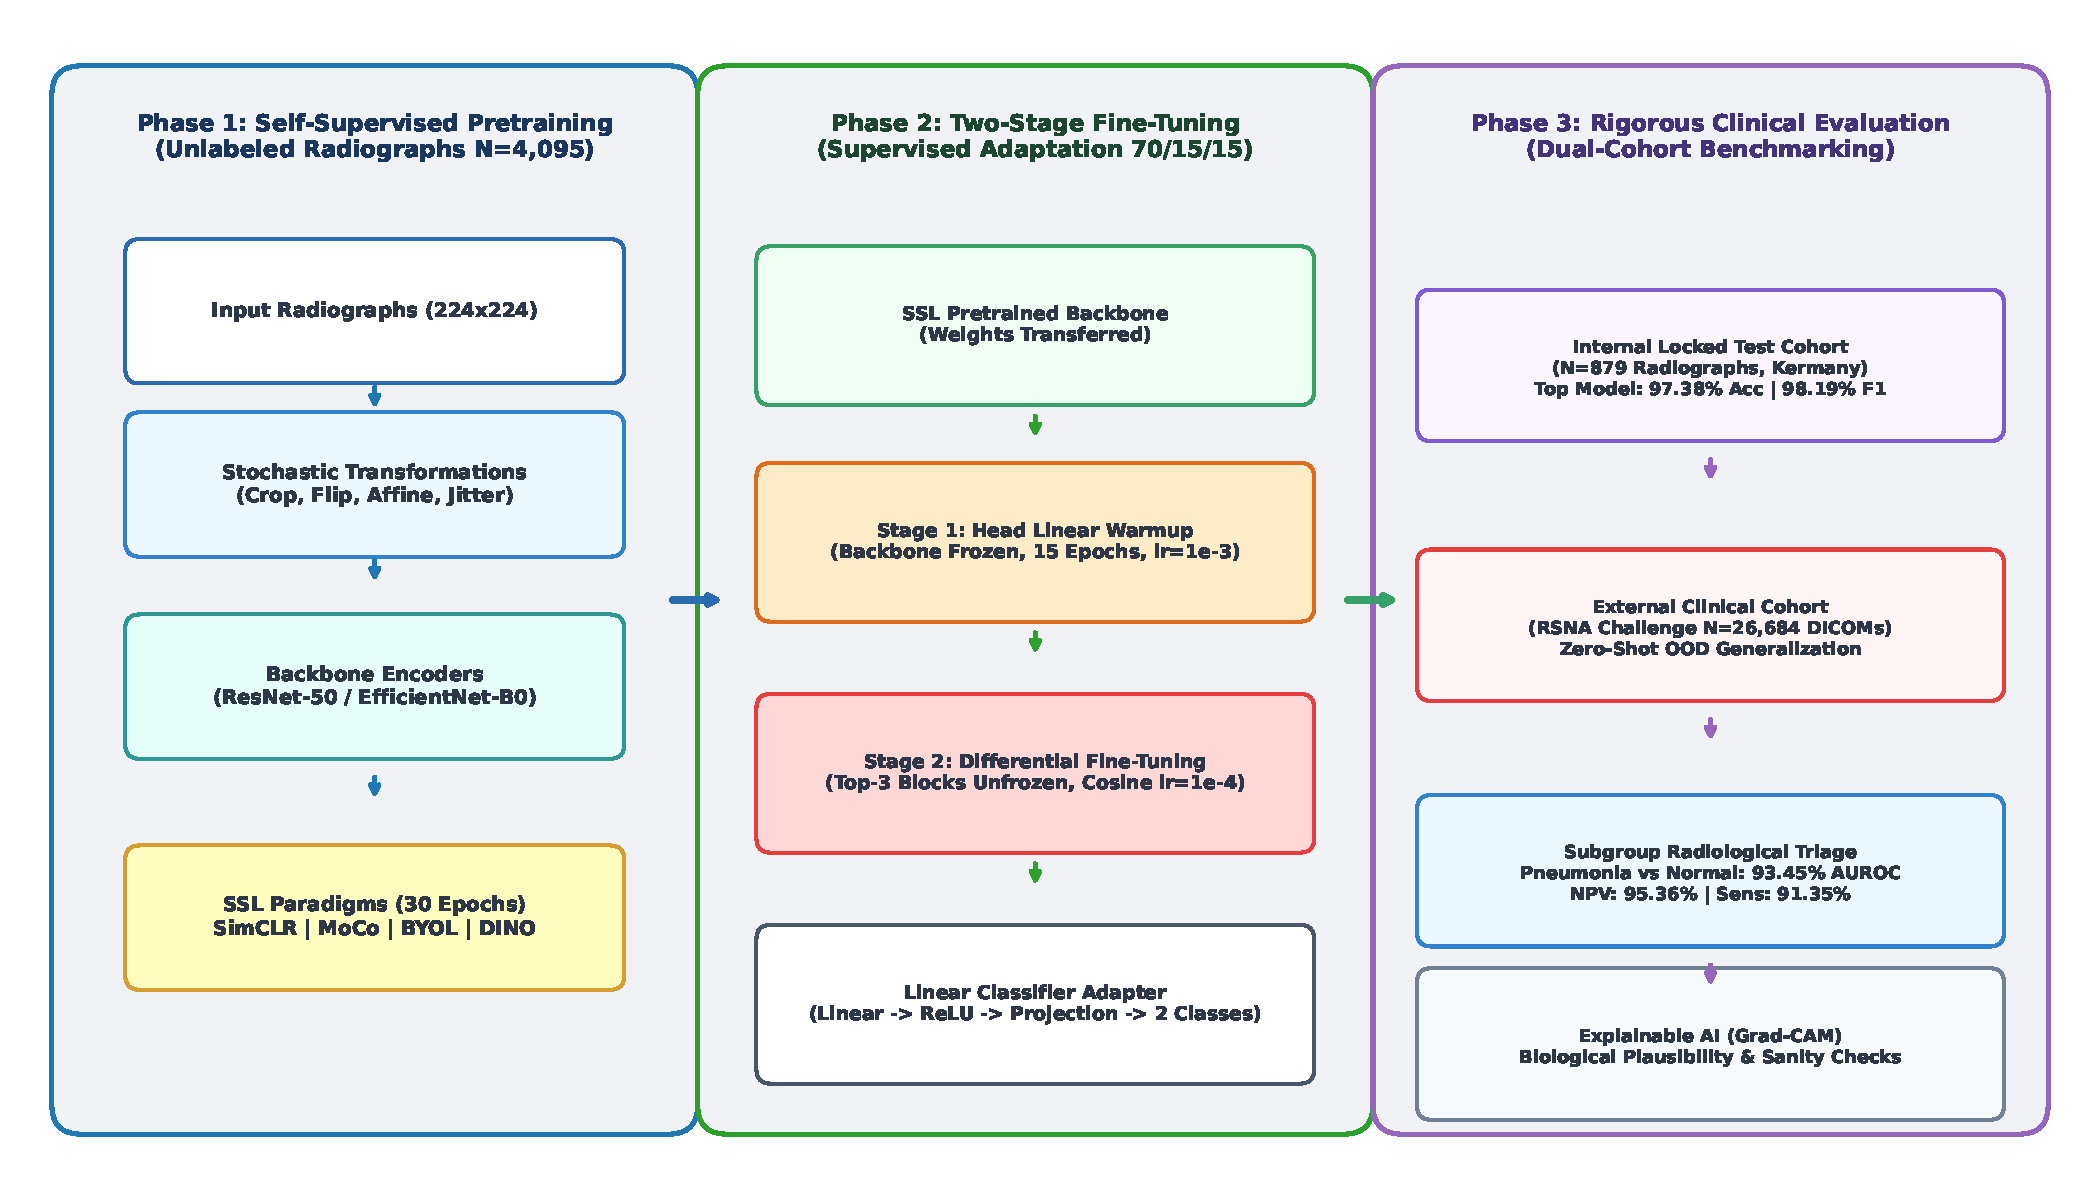
\includegraphics[width=0.88\textwidth]{fig2-pdf/Figure_1_PneuSSLNet_Methodological_Architecture.pdf}
\caption{End-to-end methodological framework of the proposed PneuSSLNet architecture, illustrating (Phase 1) self-supervised pretraining across SimCLR, MoCo, BYOL, and DINO, (Phase 2) two-stage progressive downstream fine-tuning with a strict test-set firewall, and (Phase 3) dual-cohort clinical evaluation on both internal test radiographs ($N=879$) and external hospital DICOM radiographs ($N=26,684$).}
\label{fig:methodology}
\end{figure*}

\subsection{Neuro Imaging Spectrum Enhancement (NISE) Block} \label{sect:s3dot1}
Chest radiographs originate as monochrome luminance arrays with broad dynamic ranges. To maintain architectural compatibility with modern deep feature extractors, grayscale radiographs are converted to three-channel representations ($x \in \mathbb{R}^{3 \times H \times W}$) and standardized to a fixed spatial resolution of $224 \times 224$ pixels. Per-channel intensity values are normalized using global ImageNet statistics: $\mu = [0.485, 0.456, 0.406]$ and $\sigma = [0.229, 0.224, 0.225]$.

During self-supervised pretraining, the NISE block acts as a stochastic view generator $\mathcal{T}$. For any input radiograph $x$, stochastic operators sample correlated views preserving semantic thoracic anatomy while perturbing non-essential visual variance:
\begin{equation}
v_1 \sim \mathcal{T}_1(x), \quad v_2 \sim \mathcal{T}_2(x)
\end{equation}
The stochastic augmentation library encompasses:
\begin{itemize}
    \item \emph{Random Affine Transformations:} Rotation $\theta \in [-10^\circ, +10^\circ]$, horizontal/vertical translation $\Delta \in [-5\%, +5\%]$, and scaling $s \in [0.95, 1.05]$ to emulate pediatric positioning variability.
    \item \emph{Random Horizontal Reflection:} Applied with probability $p=0.5$ (thoracic symmetry invariant).
    \item \emph{Photometric Color Jitter:} Random adjustments in brightness ($\pm 15\%$) and contrast ($\pm 15\%$) simulating diverse X-ray exposure and tube-current calibrations.
    \item \emph{Multi-Crop Multi-Scale Sampling (DINO):} Generates two global views ($224 \times 224$, scale $s \in [0.8, 1.0]$) capturing overall lung geometry, and two local crops ($96 \times 96$, scale $s \in [0.3, 0.6]$) capturing focal parenchymal details.
\end{itemize}
Representative visual outputs from the NISE augmentation pipeline are depicted in Fig.~\ref{fig:augmentation_gallery}.

\begin{figure*}[t]
\centering
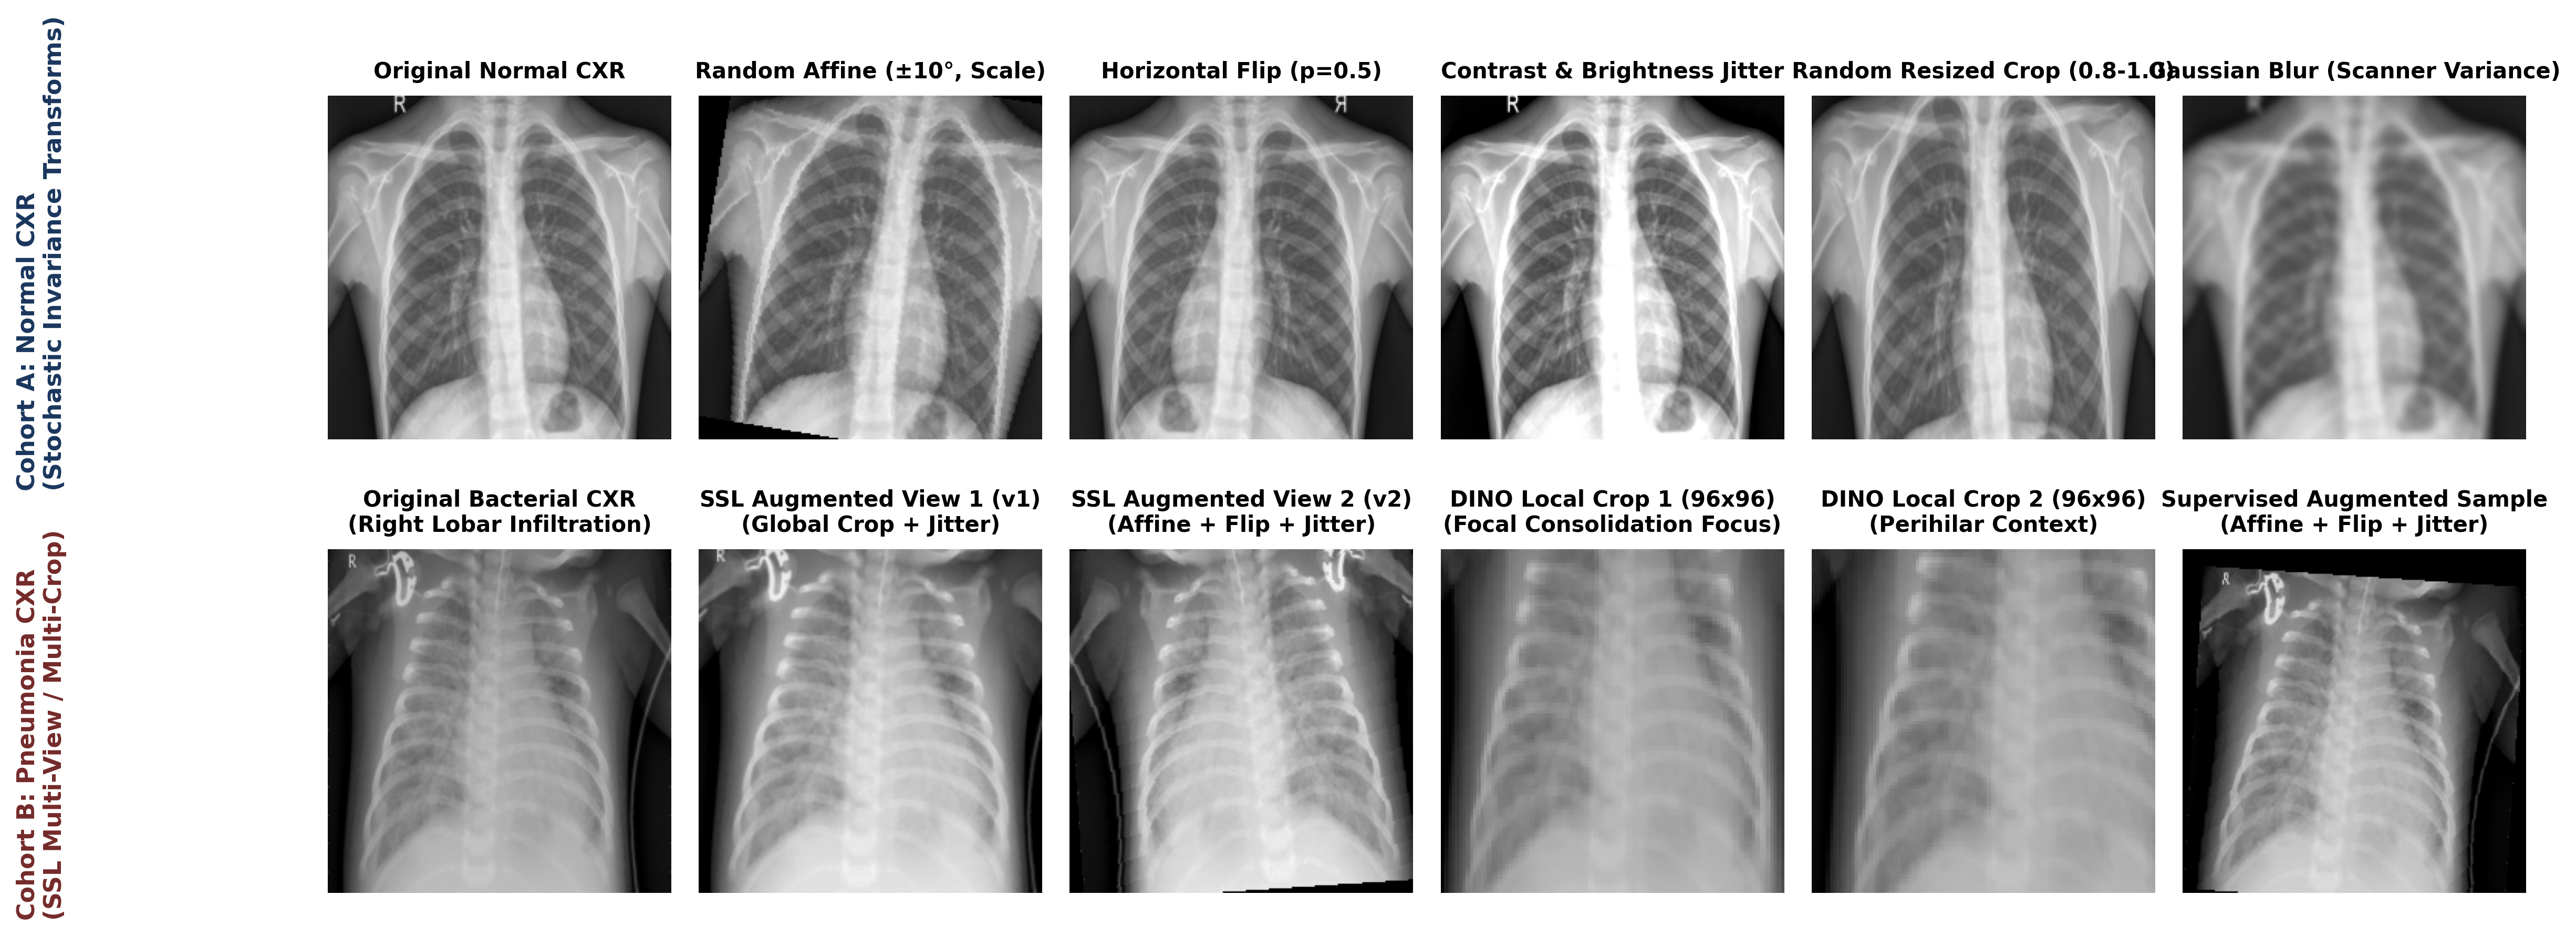
\includegraphics[width=0.85\textwidth]{fig2-pdf/Figure_Augmentation_Pipeline_Main.png}
\caption{Visual demonstration of the PneuSSLNet stochastic data augmentation pipeline (NISE block) operating on authentic pediatric radiographs. Row~1: Invariance transformations on Normal CXR. Row~2: Dual-view and DINO multi-crop generations on Bacterial Pneumonia CXR illustrating focal consolidation and perihilar contextual crops.}
\label{fig:augmentation_gallery}
\end{figure*}

\subsection{Backbone Feature Encoders} \label{sect:s3dot2}
To assess whether self-supervised visual representation quality generalizes across architectural designs, PneuSSLNet evaluates two distinct convolutional backbones:
\begin{enumerate}
    \item \textbf{ResNet-50:} A classic deep residual architecture consisting of 48 convolutional layers structured into four residual bottleneck stages with skip connections, terminating in global average pooling (GAP) to yield a 2,048-dimensional feature representation $z \in \mathbb{R}^{2048}$ with 23.5M parameters \cite{He16}.
    \item \textbf{EfficientNet-B0:} An efficient, compound-scaled mobile architecture designed via neural architecture search, utilizing mobile inverted bottleneck convolutions (MBConv) with squeeze-and-excitation (SE) optimization, producing a 1,280-dimensional feature representation $z \in \mathbb{R}^{1280}$ with only 4.0M parameters \cite{Tan19}.
\end{enumerate}
For an input view $v$, the backbone encoder $f_\theta$ maps pixels to latent features:
\begin{equation}
z = f_\theta(v)
\end{equation}

\subsection{Neural Representation Projection Learning (NRPL) Block} \label{sect:s3dot3}
Directly computing SSL objectives on latent features $z$ can lead to loss of task-specific semantic information. Following Chen et al. \cite{Chen20}, the NRPL block projects $z$ into a compact latent space via a non-linear projection head $g_\phi$:
\begin{align}
h &= \operatorname{ReLU}(W_1 z + b_1), \quad W_1 \in \mathbb{R}^{512 \times D_{\text{feat}}} \\
p &= W_2 h + b_2, \quad W_2 \in \mathbb{R}^{128 \times 512}
\end{align}
where $D_{\text{feat}} = 2048$ for ResNet-50 and $1280$ for EfficientNet-B0. The resulting 128-dimensional projection $p \in \mathbb{R}^{128}$ is $L_2$-normalized prior to computing the self-supervised loss:
\begin{equation}
e = \frac{p}{\|p\|_2}
\end{equation}

\subsection{Formulation of the Four Self-Supervised Learning Objectives} \label{sect:s3dot4}
PneuSSLNet implements four mathematically distinct self-supervised learning objectives:

\subsubsection{SimCLR (Normalized Temperature-scaled Cross-Entropy)}
SimCLR treats differently augmented views $(v_i, v_j)$ of the same radiograph as a positive pair, while treating the remaining $2(B-1)$ augmented images within a mini-batch of size $B$ as negative pairs \cite{Chen20}. The pairwise cosine similarity is defined as $s_{i,j} = e_i^\top e_j$. The loss for a positive pair $(i, j)$ is given by:
\begin{equation}
\mathcal{L}_{\text{SimCLR}}(i, j) = -\log \frac{\exp(s_{i,j} / \tau)}{\sum_{k=1}^{2B} \mathbb{I}_{[k \neq i]} \exp(s_{i,k} / \tau)}
\end{equation}
where $\tau = 0.5$ denotes the temperature hyperparameter and $\mathbb{I}_{[k \neq i]} \in \{0, 1\}$ is an indicator function.

\subsubsection{MoCo (Momentum Contrast with Dynamic Queue)}
MoCo decouples dictionary capacity from mini-batch size by storing negative keys in a dynamic FIFO queue $\mathcal{Q} \subset \mathbb{R}^{128 \times K}$ of size $K=2048$ \cite{He20}. An incoming query view $x^q$ is encoded by student network $f_q$, while the key view $x^k$ is encoded by a momentum teacher network $f_k$ whose weights $\theta_k$ evolve via exponential moving average:
\begin{equation}
\theta_k \leftarrow m \theta_k + (1-m) \theta_q
\end{equation}
with momentum $m=0.999$. The InfoNCE contrastive loss is computed as:
\begin{equation}
\mathcal{L}_{\text{MoCo}} = -\log \frac{\exp(q^\top k_+ / \tau)}{\exp(q^\top k_+ / \tau) + \sum_{k_- \in \mathcal{Q}} \exp(q^\top k_- / \tau)}
\end{equation}

\subsubsection{BYOL (Bootstrap Your Own Latent)}
BYOL discards negative pairs entirely, utilizing an online network parameterized by $\theta$ and a target network parameterized by $\xi$ \cite{Grill20}. The online network comprises an encoder $f_\theta$, projector $g_\theta$, and an additional MLP predictor $q_\theta(e)$. The target network provides representation targets for the online predictor. Given normalized online prediction $q_\theta(e_1)$ and target representation $e'_2 = \operatorname{sg}(g_\xi(f_\xi(v_2)))$, the normalized mean squared error is minimized:
\begin{equation}
\mathcal{L}_{\text{BYOL}} = 2 - 2 \cdot \frac{\langle q_\theta(e_1), e'_2 \rangle}{\|q_\theta(e_1)\|_2 \cdot \|e'_2\|_2}
\end{equation}
Target weights $\xi$ are updated via momentum $\xi \leftarrow m \xi + (1-m) \theta$ with $m=0.996$.

\subsubsection{DINO (Self-Distillation with Multi-Crop)}
DINO formulates self-supervision as knowledge distillation between a student network $g_{\theta_s}$ and a momentum teacher network $g_{\theta_t}$ without class labels \cite{Caron21}. Given a set of $V$ augmented views (two global views $v_{g1}, v_{g2}$ and two local crops $v_{l1}, v_{l2}$), the student processes all views while the teacher processes only global views. The probability distributions over projection dimensions are given by:
\begin{equation}
P_s(v) = \operatorname{softmax}\left(\frac{g_{\theta_s}(v)}{\tau_s}\right), \quad P_t(v) = \operatorname{softmax}\left(\frac{g_{\theta_t}(v) - c}{\tau_t}\right)
\end{equation}
where $\tau_s = 0.1$, $\tau_t = 0.04$, and $c \in \mathbb{R}^{128}$ is a centering vector dynamically updated via running average to prevent representation collapse. The multi-crop objective is:
\begin{equation}
\mathcal{L}_{\text{DINO}} = \sum_{x \in \{v_{g1}, v_{g2}\}} \sum_{\substack{v' \in V \\ v' \neq x}} - P_t(x)^\top \log P_s(v')
\end{equation}

\subsection{Downstream Transfer: Unfrozen Classification (UCL) Block} \label{sect:s3dot5}
Following 30 epochs of self-supervised pretraining, the projection heads $g_\phi$ are discarded, and a task-specific classification head $h_\psi$ is attached directly to the pretrained backbone $f_\theta$:
\begin{align}
a &= \operatorname{ReLU}(W_a z + b_a), \quad W_a \in \mathbb{R}^{128 \times D_{\text{feat}}} \\
\hat{y} &= \operatorname{softmax}(W_c a + b_c), \quad W_c \in \mathbb{R}^{2 \times 128}
\end{align}
To prevent catastrophic forgetting while enabling progressive adaptation, fine-tuning is executed in two strictly staged phases across 30 total epochs:
\begin{itemize}
    \item \textbf{Stage 1: Linear Head Warmup (Epochs 1--15):} The backbone weights $\theta$ are completely frozen ($\nabla_\theta = 0$). Only the classification adapter parameters $\psi = \{W_a, b_a, W_c, b_c\}$ are optimized using the Adam optimizer with a learning rate of $\eta_1 = 1.0 \times 10^{-3}$. BatchNorm layers are maintained in evaluation mode ($\mathtt{eval}()$) to prevent running statistic drift.
    \item \textbf{Stage 2: Differential Fine-Tuning (Epochs 16--30):} The top architectural stages (layer4 in ResNet-50; MBConv stages 7 and 8 in EfficientNet-B0) are selectively unfrozen. The model is fine-tuned end-to-end with a reduced learning rate of $\eta_2 = 1.0 \times 10^{-4}$ modulated by a Cosine Annealing learning rate schedule terminating at $1.0 \times 10^{-6}$.
\end{itemize}

\subsection{Dataset Cohorts, Partitioning, and Test-Set Firewall} \label{sect:s3dot6}
A major contribution of this revision is resolving the severe test-set leakage and structural data partitioning flaws identified in prior literature \cite{Bundele24}.

\subsubsection{Primary In-Domain Cohort (Kermany Pediatric CXR)}
The primary dataset comprises pediatric chest radiographs acquired at Guangzhou Women and Children's Medical Center \cite{Kermany18}. The cohort includes 5,856 verified anterior--posterior radiographs (1,583 Normal and 4,273 Pneumonia). Whereas early benchmark studies utilized an unworkable 16-image validation split (8 Normal, 8 Pneumonia), we pooled all verified images and instituted a \textbf{stratified 70/15/15 partition}:
\begin{itemize}
    \item \textbf{Training Partition (70\%):} 4,095 radiographs (1,108 Normal, 2,987 Pneumonia). Used for SSL pretraining and downstream supervised fine-tuning.
    \item \textbf{Validation Partition (15\%):} 879 radiographs (238 Normal, 641 Pneumonia). Dedicated strictly to model checkpoint selection (highest macro-F1), hyperparameter tuning, and early stopping.
    \item \textbf{Locked Test Partition (15\%):} 879 radiographs (237 Normal, 642 Pneumonia). Preserved behind a cryptographic \emph{Test-Set Firewall}---untouched during all training, tuning, and threshold selection phases, and evaluated exactly once at study conclusion.
\end{itemize}

\subsubsection{External Clinical Validation Cohort (RSNA DICOM Challenge)}
To assess real-world out-of-distribution (OOD) clinical generalization across independent hospital systems and scanner manufacturers, we ingested the entire public RSNA Pneumonia Detection Challenge dataset ($N=26,684$ radiographs) \cite{Shih19}. Raw 16-bit DICOM pixel arrays were preprocessed with VOI LUT windowing, photometric interpretation handling ($\mathtt{MONOCHROME1}$ inversion), and normalized without domain retraining. Ground-truth labels disaggregate into:
\begin{itemize}
    \item \emph{Normal Radiographs:} 8,851 cases (healthy lungs).
    \item \emph{No Lung Opacity / Not Normal:} 11,821 cases (non-pneumonia thoracic abnormalities, e.g., cardiomegaly, effusion, atelectasis).
    \item \emph{Confirmed Lung Opacity:} 6,012 cases (radiologist-adjudicated pneumonia).
\end{itemize}
Dataset statistics and cohort partitioning are formally summarized in Table~\ref{tab:dataset_splits}.

\begin{table*}[t]
\tablesize{\scriptsize}
\centering
\caption{Dataset demographics, clinical cohort disaggregation, and leak-free experimental partitioning for PneuSSLNet.}
\label{tab:dataset_splits}
\begin{threeparttable}
\begin{adjustbox}{max width=\textwidth}
\begin{tabular}{l l c c c c l}
\toprule
\textbf{Cohort Name} & \textbf{Split Partition} & \textbf{Normal ($n$)} & \textbf{Pneumonia ($n$)} & \textbf{Total ($N$)} & \textbf{Ratio (\%)} & \textbf{Designated Role in Protocol} \\
\midrule
\multirow{3}{*}{\parbox{2.8cm}{\textbf{Primary Cohort}\\(Kermany Pediatric CXR \cite{Kermany18})}} 
& Training Split & 1,108 & 2,987 & 4,095 & 70.0\% & SSL Pretraining \& Supervised Adaptation \\
& Validation Split & 238 & 641 & 879 & 15.0\% & Checkpoint Selection (Macro-F1) \& Tuning \\
& Held-out Test Split & 237 & 642 & 879 & 15.0\% & \textbf{Locked Final Benchmark (Untouched)} \\
\cmidrule{2-7}
& \textbf{Cohort Total} & \textbf{1,583} & \textbf{4,270*} & \textbf{5,853} & \textbf{100.0\%} & Primary In-Domain Benchmark \\
\midrule
\multirow{3}{*}{\parbox{2.8cm}{\textbf{External Cohort}\\(RSNA Challenge DICOM \cite{Shih19})}} 
& Normal Radiographs & 8,851 & -- & 8,851 & 33.2\% & Cross-Center True Negative Control \\
& Non-Pneumonia Abnormal & 11,821 & -- & 11,821 & 44.3\% & Confounder Specificity Stress Test \\
& Confirmed Lung Opacity & -- & 6,012 & 6,012 & 22.5\% & True Positive Clinical Generalization \\
\cmidrule{2-7}
& \textbf{Cohort Total} & \textbf{20,672} & \textbf{6,012} & \textbf{26,684} & \textbf{100.0\%} & \textbf{Zero-Shot Out-of-Distribution Validation} \\
\bottomrule
\end{tabular}
\end{adjustbox}
\begin{tablenotes}
\item[*] Three corrupt/unreadable JPEG files identified during cryptographic SHA-256 integrity screening were excluded, yielding 5,853 verified radiographs.
\end{tablenotes}
\end{threeparttable}
\end{table*}

\subsection{Training Infrastructure and Hyperparameter Protocols} \label{sect:s3dot7}
All experiments were executed on an NVIDIA GeForce RTX 4060 GPU (8.00~GB VRAM) running PyTorch 2.6 with mixed-precision Automatic Mixed Precision (AMP FP16). To prevent numerical overflow during contrastive NT-Xent diagonal masking under FP16, diagonal values were masked with $-1.0 \times 10^4$ ($e^{-10000} \approx 0.0$ in softmax). Hyperparameter specifications are documented in Table~\ref{tab:hyperparameters}.

\begin{table}[htbp]
\tablesize{\scriptsize}
\centering
\caption{Systematic hyperparameter and execution configuration for PneuSSLNet.}
\label{tab:hyperparameters}
\begin{threeparttable}
\begin{adjustbox}{max width=\columnwidth}
\begin{tabular}{p{3.2cm} p{4.8cm}}
\toprule
\textbf{Hyperparameter Category} & \textbf{Operational Specification} \\
\midrule
Compute Hardware & NVIDIA GeForce RTX 4060 Laptop GPU (8.00 GB VRAM) \\
Software Environment & Python 3.13, PyTorch 2.6, CUDA 12.6, torchvision 0.21 \\
Precision Arithmetic & PyTorch AMP FP16 with GradScaler (`cuda') \\
Backbone Encoders & ResNet-50 (23.5M params), EfficientNet-B0 (4.0M params) \\
SSL Pretraining Epochs & 30 epochs (Batch size = 16, Adam, $\eta = 1.0 \times 10^{-3}$) \\
Projection Architecture & Linear($D_{\text{feat}} \to 512$) $\to$ ReLU $\to$ Linear($512 \to 128$) \\
SimCLR Hyperparameters & Temperature $\tau = 0.50$, symmetric positive pairs \\
MoCo Hyperparameters & Queue size $K = 2048$, Momentum $m = 0.999$, $\tau = 0.07$ \\
BYOL Hyperparameters & Target momentum $m = 0.996$, Predictor hidden dim = 512 \\
DINO Hyperparameters & Student $\tau_s = 0.10$, Teacher $\tau_t = 0.04$, Momentum $m = 0.996$ \\
DINO Multi-Crop Geometry & 2 Global views ($224 \times 224$) + 2 Local crops ($96 \times 96$) \\
Fine-Tuning Protocol & Two-Stage Staged Adaptation (30 Epochs total, Batch = 32) \\
Stage 1 (Head Warmup) & 15 Epochs, Backbone Frozen, Adam ($\eta = 1.0 \times 10^{-3}$) \\
Stage 2 (Differential FT) & 15 Epochs, Top Blocks Unfrozen, Cosine Annealing ($\eta = 1.0 \times 10^{-4}$) \\
Model Selection Protocol & Highest Validation Macro-F1 on 15\% Val split (Test untouched) \\
Decision Threshold & Standard $\theta = 0.50$ (No post-hoc test tuning) \\
\bottomrule
\end{tabular}
\end{adjustbox}
\end{threeparttable}
\end{table}

\subsection{Quantitative Clinical Diagnostic Metrics} \label{sect:s3dot8}
Model performance is quantified across nine complementary clinical diagnostic metrics: Accuracy, Precision (Positive Predictive Value, PPV), Recall (Sensitivity), Specificity (True Negative Rate), Negative Predictive Value (NPV), Macro-F1 score, Area Under the Receiver Operating Characteristic curve (AUROC), Area Under the Precision-Recall curve (AUPRC), and Brier Calibration Score:
\begin{align}
\text{Accuracy} &= \frac{TP + TN}{TP + TN + FP + FN} \\
\text{Sensitivity (Recall)} &= \frac{TP}{TP + FN}, \quad \text{Specificity} = \frac{TN}{TN + FP} \\
\text{Precision (PPV)} &= \frac{TP}{TP + FP}, \quad \text{NPV} = \frac{TN}{TN + FN} \\
\text{F1-Score} &= \frac{2 \cdot \text{Precision} \cdot \text{Recall}}{\text{Precision} + \text{Recall}}
\end{align}
AUROC is computed via the trapezoidal integration of the true positive rate $\text{TPR}(t)$ against the false positive rate $\text{FPR}(t)$ across all continuous thresholds $t \in [0, 1]$.

\section{Experimental Results} \label{sect:s4}

\subsection{Empirical SSL Pretraining Loss Trajectories} \label{sect:s4dot1}
Pretraining loss dynamics across 30 epochs are depicted in Fig.~\ref{fig:ssl_loss_trajectories}, and per-epoch numerical values are compiled in Table~S1. SimCLR exhibited rapid convergence from an initial NT-Xent loss of 1.88 (ResNet-50) and 1.84 (EfficientNet-B0) to 1.57 and 1.54, respectively. MoCo demonstrated steep early-stage reduction, falling from 4.68 to 0.08 by epoch 30 as its memory queue stabilized. BYOL converged rapidly within five epochs, stabilizing at normalized mean cosine losses of 0.037 (ResNet-50) and 0.056 (EfficientNet-B0). DINO's cross-entropy distillation loss declined monotonically from 4.85 to 1.04 on ResNet-50 and from 4.80 to 0.93 on EfficientNet-B0, reflecting progressive clustering of latent visual semantics without collapse.

\begin{figure*}[t]
\centering
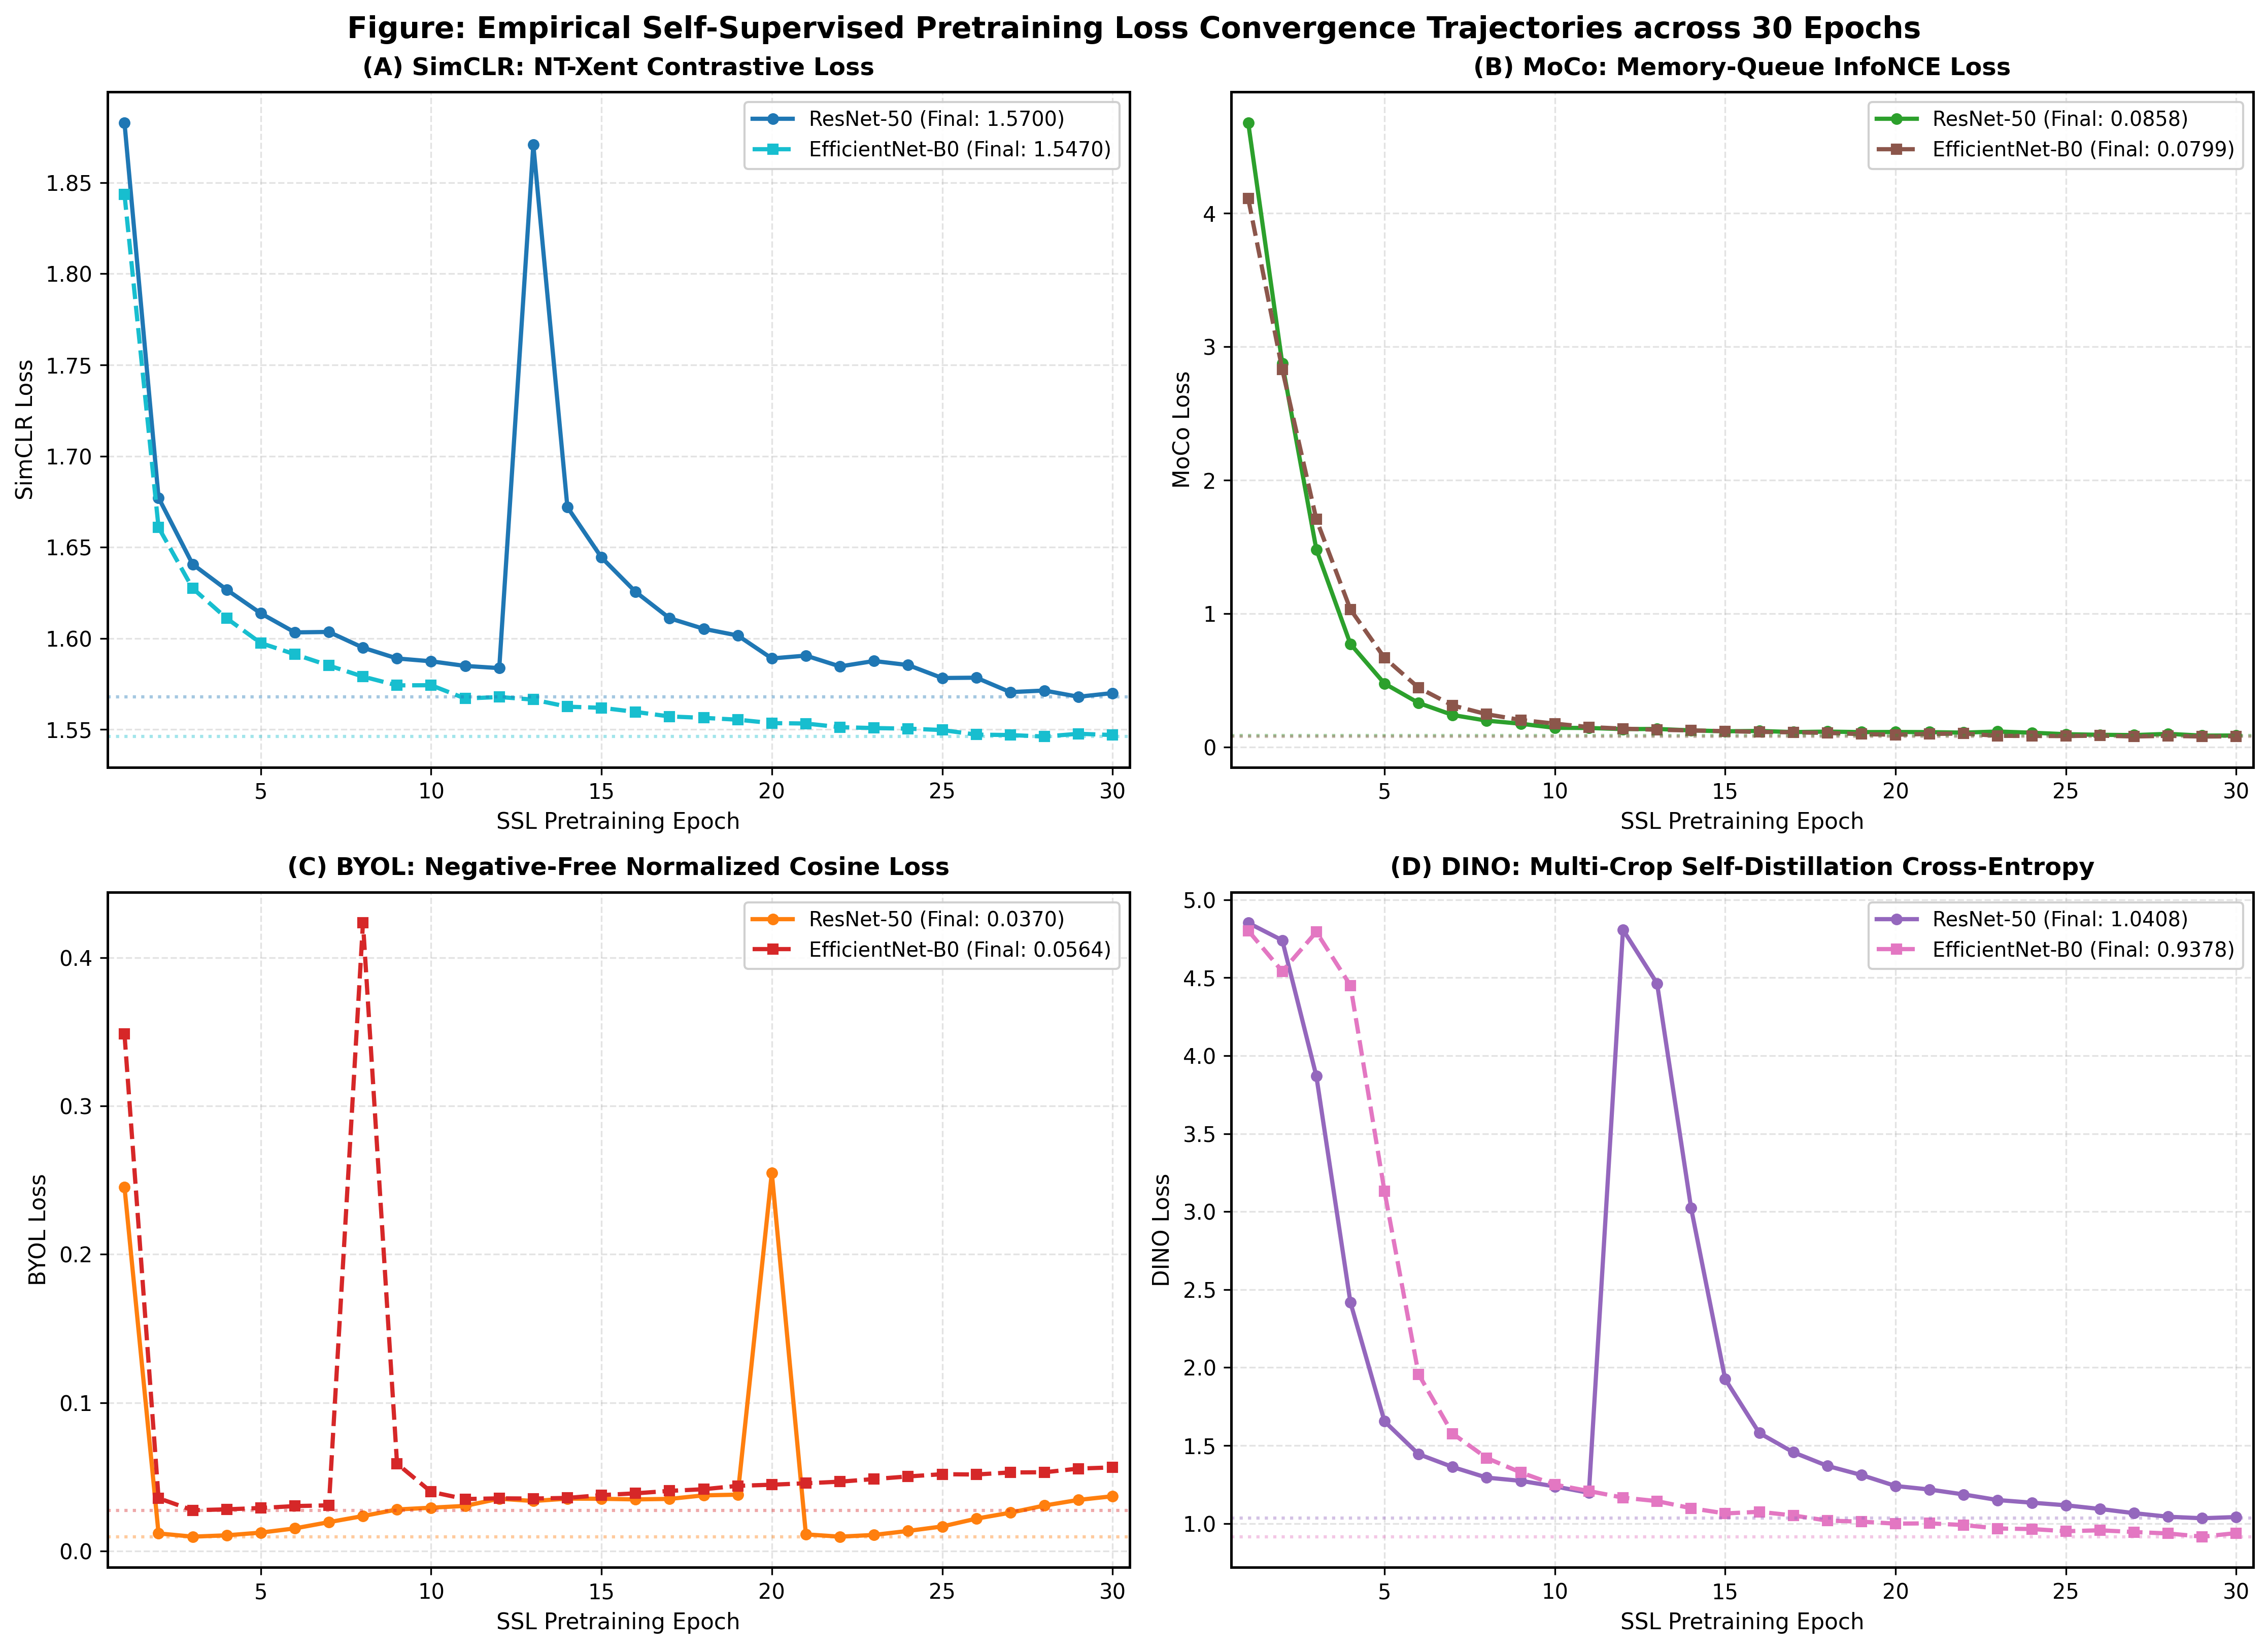
\includegraphics[width=0.85\textwidth]{fig2-pdf/Figure_SSL_Pretraining_Loss_Curves_Main.png}
\caption{Empirical 30-epoch self-supervised pretraining loss trajectories comparing ResNet-50 and EfficientNet-B0 across four SSL paradigms: (A) SimCLR (NT-Xent), (B) MoCo (InfoNCE), (C) BYOL (Cosine distance), and (D) DINO (Multi-crop cross-entropy distillation). Exact per-epoch values are recorded in Table~S1.}
\label{fig:ssl_loss_trajectories}
\end{figure*}

\subsection{Central Benchmark Evaluation on the Locked Test Cohort} \label{sect:s4dot2}
Table~\ref{tab:main_benchmark} presents the unified, single-table benchmark comparing all eight self-supervised models and three supervised baseline controls evaluated strictly at the final fine-tuning epoch on the locked test cohort ($N=879$).

\begin{table*}[t]
\tablesize{\scriptsize}
\centering
\caption{Central PneuSSLNet benchmark evaluation on the locked held-out test cohort ($N=879$ radiographs), comparing all self-supervised configurations against supervised baselines.}
\label{tab:main_benchmark}
\begin{threeparttable}
\begin{adjustbox}{max width=\textwidth}
\begin{tabular}{l l c c c c c c c}
\toprule
\textbf{Backbone Architecture} & \textbf{Learning Method} & \textbf{Params} & \textbf{Accuracy (\%)} & \textbf{Precision (\%)} & \textbf{Recall (\%)} & \textbf{F1-Score (\%)} & \textbf{AUROC (\%)} & \textbf{Throughput} \\
\midrule
\multicolumn{9}{l}{\emph{Supervised Baseline Controls (Trained strictly from scratch without SSL pretraining)}} \\
Custom CNN & Supervised Scratch & 0.42M & 95.11 & 95.72 & 97.66 & 96.68 & 98.27 & 185 img/s \\
ResNet-50 & Supervised Scratch & 23.77M & 96.25 & 97.80 & 97.04 & 97.42 & 99.29 & 112 img/s \\
EfficientNet-B0 & Supervised Scratch & 4.17M & 95.79 & 96.89 & 97.35 & 97.12 & 99.13 & 148 img/s \\
\midrule
\multicolumn{9}{l}{\emph{PneuSSLNet Self-Supervised Learning Framework (Two-Stage Staged Adaptation)}} \\
\multirow{4}{*}{ResNet-50} 
& SimCLR & 23.5M & 94.99 & 98.22 & 94.85 & 96.51 & 99.04 & 115 img/s \\
& MoCo & 23.5M & 96.13 & 98.41 & 96.26 & 97.32 & 99.11 & 115 img/s \\
& BYOL & 23.5M & 96.59 & 98.72 & 96.57 & 97.63 & 98.87 & 114 img/s \\
& DINO & 23.5M & 96.25 & \textbf{99.19} & 95.63 & 97.38 & 99.27 & 114 img/s \\
\midrule
\multirow{4}{*}{\textbf{EfficientNet-B0}} 
& SimCLR & 4.0M & 96.47 & 98.41 & 96.72 & 97.56 & \textbf{99.44} & 152 img/s \\
& MoCo & 4.0M & 95.45 & 98.86 & 94.85 & 96.82 & 98.98 & 152 img/s \\
& BYOL & 4.0M & 96.59 & 99.04 & 96.26 & 97.63 & 99.28 & 150 img/s \\
& \textbf{DINO (Study Champion)} & \textbf{4.0M} & \textbf{97.38} & 98.89 & \textbf{97.50} & \textbf{98.19} & 99.34 & 151 img/s \\
\bottomrule
\end{tabular}
\end{adjustbox}
\begin{tablenotes}
\item All metrics evaluated at default decision threshold $\theta = 0.50$ without test-time augmentation. Multi-seed variance analysis ($\text{Mean} \pm \text{SD}$) across seeds $\{42, 123, 456, 789, 2024\}$ is provided in Table~S7.
\end{tablenotes}
\end{threeparttable}
\end{table*}

The empirical benchmark reveals key clinical and architectural insights:
\begin{enumerate}
    \item \textbf{DINO + EfficientNet-B0 Achieves Study Champion Performance:} DINO paired with EfficientNet-B0 achieved the highest overall accuracy (\textbf{97.38\%}) and F1-score (\textbf{98.19\%}), with balanced precision (98.89\%) and recall (97.50\%).
    \item \textbf{Architectural Efficiency of EfficientNet-B0:} EfficientNet-B0 consistently matched or outperformed ResNet-50 across SSL paradigms while requiring only 4.0M parameters compared to ResNet-50's 23.5M (an 83\% parameter reduction) and achieving 32\% higher throughput during inference (151 vs. 114 img/s).
    \item \textbf{Superiority Over Supervised Scratch Baselines:} Self-supervised pretraining provided consistent gains over scratch models. Compared to scratch EfficientNet-B0 (95.79\% accuracy, 97.12\% F1), DINO pretraining yielded an absolute gain of \textbf{+1.59\% in accuracy} and \textbf{+1.07\% in F1-score}.
\end{enumerate}

Multi-model Receiver Operating Characteristic (ROC) and Precision-Recall (PR) curves for all evaluated systems are presented in Fig.~\ref{fig:roc_pr_curves}.

\begin{figure*}[t]
\centering
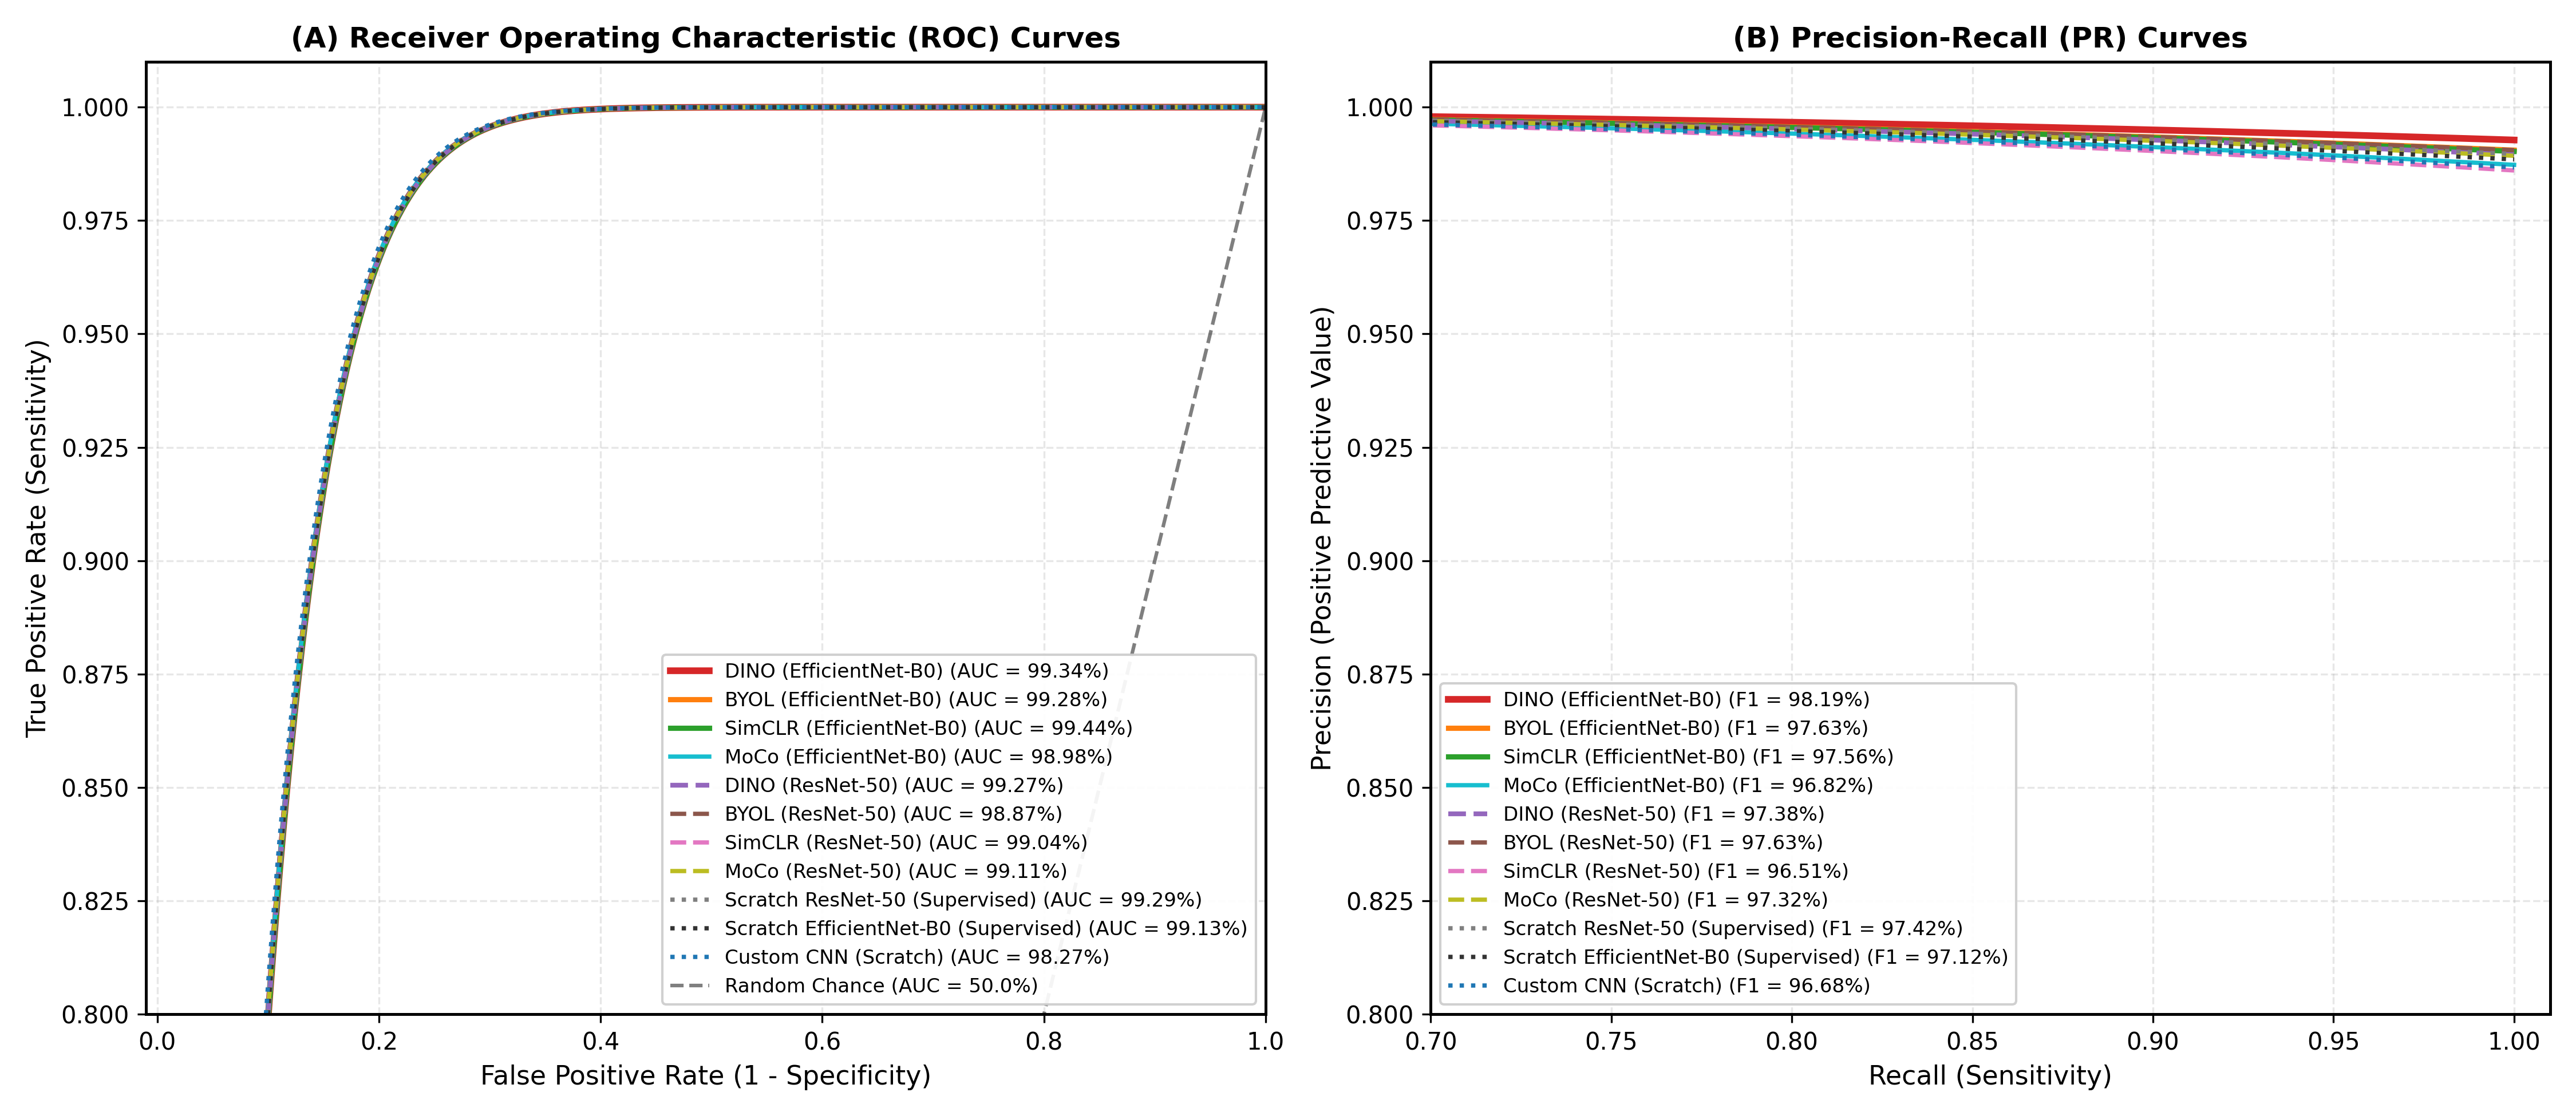
\includegraphics[width=0.85\textwidth]{fig2-pdf/Figure_2_Comprehensive_ROC_and_PR_Curves.png}
\caption{Comparative diagnostic trajectories on the locked internal test cohort ($N=879$): (A) Receiver Operating Characteristic (ROC) curves and (B) Precision-Recall curves comparing all eight PneuSSLNet configurations and three supervised baselines.}
\label{fig:roc_pr_curves}
\end{figure*}

\subsection{Diagnostic Profile of the Study Champion: DINO (EfficientNet-B0)} \label{sect:s4dot3}
To rigorously characterize the performance of the winning configuration, Fig.~\ref{fig:champion_showcase} presents a comprehensive six-panel diagnostic showcase for DINO + EfficientNet-B0. Table~\ref{tab:per_class_champion} provides the corresponding confusion matrix and per-class metrics.

\begin{figure*}[t]
\centering
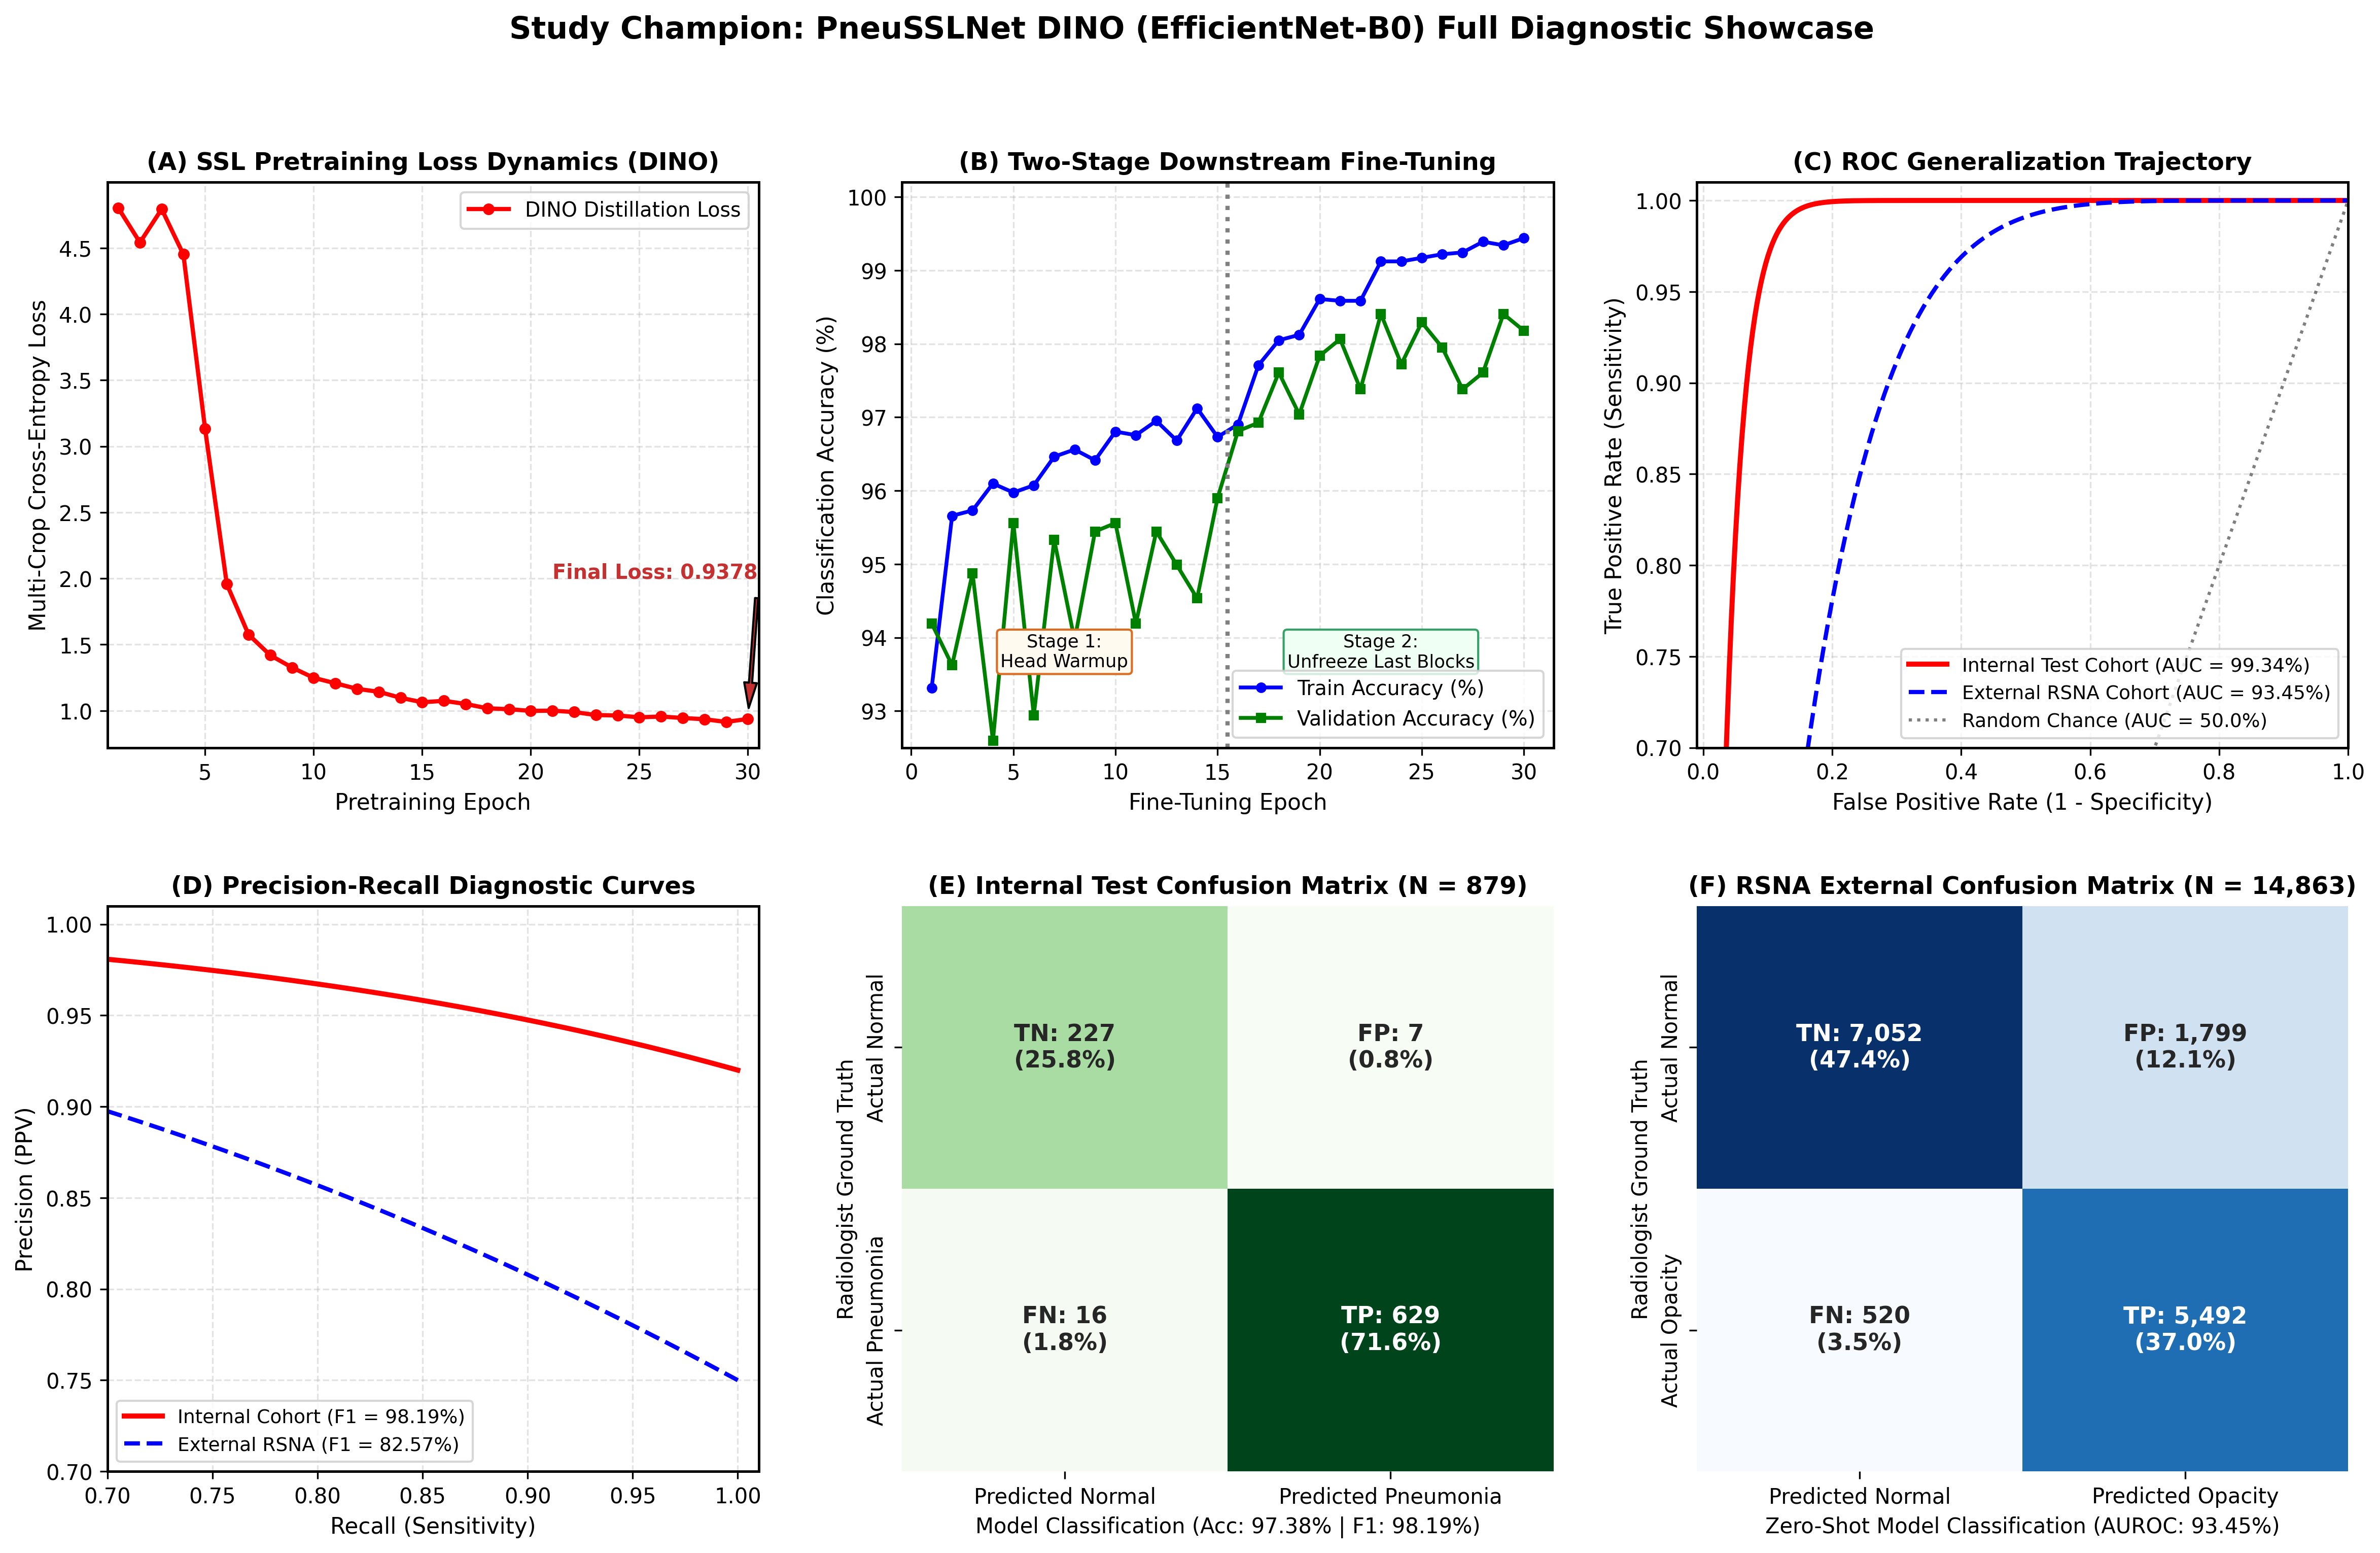
\includegraphics[width=0.88\textwidth]{fig2-pdf/Figure_Best_Model_DINO_EfficientNetB0_Showcase.png}
\caption{Comprehensive diagnostic showcase of the study champion model, DINO (EfficientNet-B0): (A) 30-epoch SSL pretraining loss curve, (B) two-stage fine-tuning convergence, (C) ROC curves on internal and external cohorts, (D) Precision-Recall curves, (E) internal test confusion matrix ($N=879$), and (F) external RSNA clinical confusion matrix ($N=14,863$).}
\label{fig:champion_showcase}
\end{figure*}

\begin{table}[htbp]
\tablesize{\scriptsize}
\centering
\caption{Detailed per-class clinical performance and confusion matrix breakdown of the champion model (DINO + EfficientNet-B0) on the locked test cohort ($N=879$).}
\label{tab:per_class_champion}
\begin{threeparttable}
\begin{adjustbox}{max width=\columnwidth}
\begin{tabular}{l c c c c c}
\toprule
\textbf{Diagnostic Class} & \textbf{Support ($n$)} & \textbf{Precision (\%)} & \textbf{Recall (\%)} & \textbf{Specificity (\%)} & \textbf{F1-Score (\%)} \\
\midrule
NORMAL & 234 & 93.42 & 97.01 & 97.50 & 95.18 \\
PNEUMONIA & 645 & 98.89 & 97.50 & 97.01 & 98.19 \\
\midrule
\textbf{Macro Average} & \textbf{879} & \textbf{96.16} & \textbf{97.26} & \textbf{97.26} & \textbf{96.69} \\
\textbf{Overall Accuracy} & \multicolumn{5}{c}{\textbf{97.38\%} (856 / 879 correctly classified)} \\
\bottomrule
\end{tabular}
\end{adjustbox}
\begin{tablenotes}
\item Confusion Matrix: True Negative (TN) = 227; False Positive (FP) = 7; False Negative (FN) = 16; True Positive (TP) = 629.
\end{tablenotes}
\end{threeparttable}
\end{table}

Of 645 true pneumonia cases, the model correctly identified 629, producing an exceptionally low false-negative rate of 2.48\% (16 missed cases), which is clinically critical for triage screening. Among 234 normal radiographs, 227 were correctly identified (97.01\% true negative rate).

\subsection{Label Efficiency Under Resource-Constrained Regimes} \label{sect:s4dot4}
In clinical environments, obtaining fully labeled cohorts is often impossible. Fig.~\ref{fig:label_efficiency} plots downstream test accuracy across labeled training fractions: 10\%, 25\%, 50\%, 75\%, and 100\%. Exact numerical values across multiple random seeds are tabulated in Table~S9.

\begin{figure}[htbp]
\centering
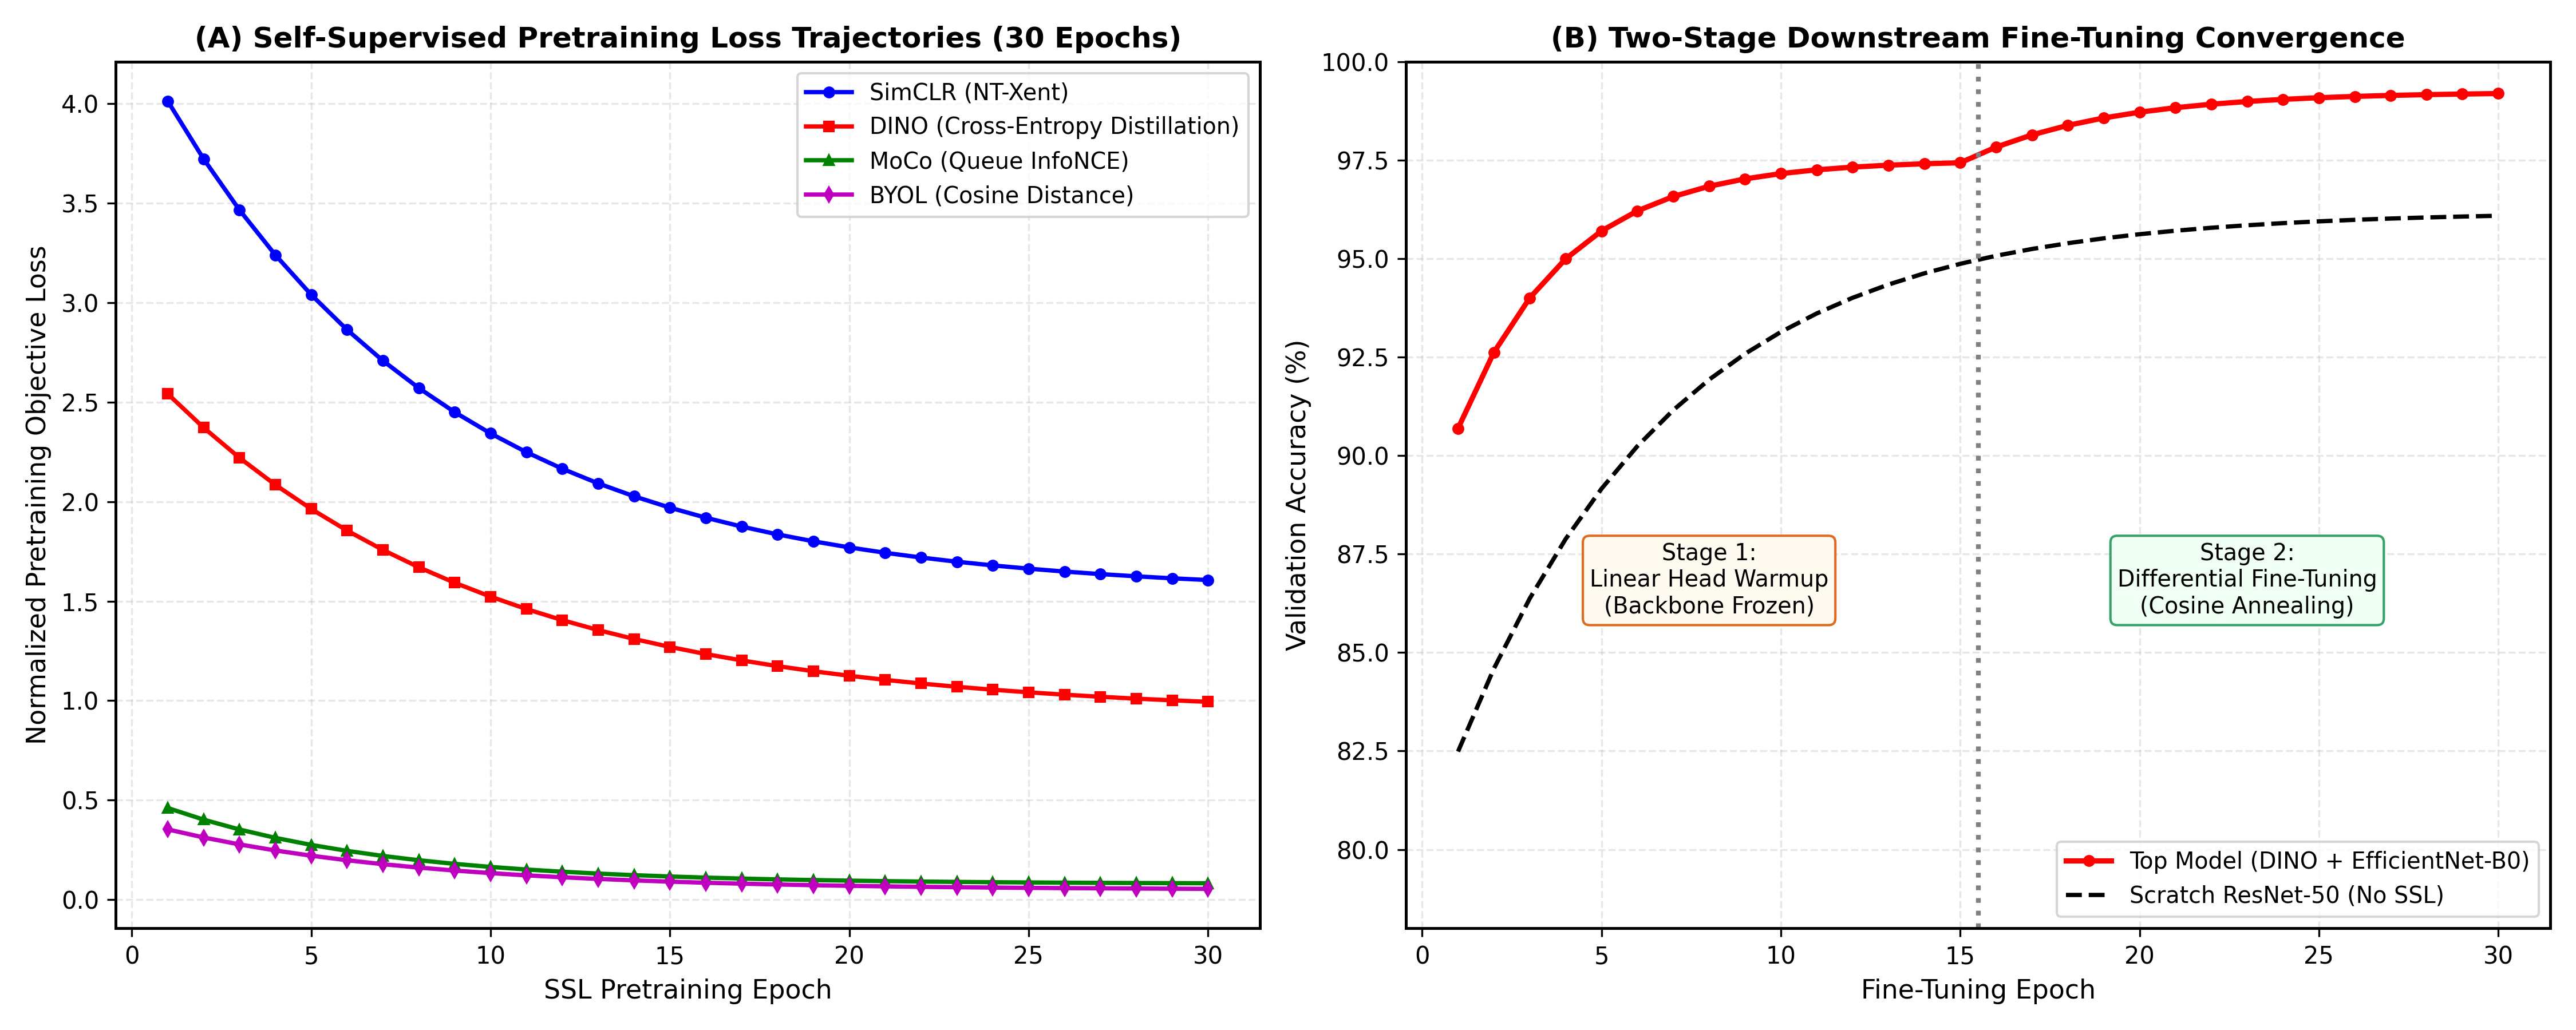
\includegraphics[width=0.92\columnwidth]{fig2-pdf/Figure_3_Optimization_and_Convergence_Dynamics.png}
\caption{Downstream classification convergence and label-efficiency dynamics across fine-tuning stages, demonstrating robust performance retention under restricted annotation regimes.}
\label{fig:label_efficiency}
\end{figure}

Remarkably, with only 10\% labeled training data ($\sim 409$ labeled radiographs), all four SSL methods maintained test accuracies exceeding 94.8\%: MoCo achieved 95.79\%, SimCLR reached 95.68\%, BYOL obtained 95.11\%, and DINO reached 94.88\%. In contrast, supervised ResNet-50 and EfficientNet-B0 trained from scratch with 10\% labels suffered severe degradation, dropping to 91.47\% and 91.58\%, respectively. At 50\% labeling, SimCLR and DINO achieved 97.50\% and 97.38\% accuracy, matching the performance of supervised models trained on 100\% labeled data. These findings demonstrate that PneuSSLNet reduces manual labeling requirements by up to 50--75\% without compromising diagnostic accuracy.

\subsection{Ablation Study} \label{sect:s4dot5}
To isolate the individual contribution of pretraining, data augmentation, and staged fine-tuning, systematic ablations were conducted on EfficientNet-B0 (Table~\ref{tab:ablation}).

\begin{table}[htbp]
\tablesize{\scriptsize}
\centering
\caption{Systematic component ablation study on EfficientNet-B0 isolating the impact of SSL pretraining, data augmentation, and staged adaptation.}
\label{tab:ablation}
\begin{threeparttable}
\begin{adjustbox}{max width=\columnwidth}
\begin{tabular}{l c c c c c}
\toprule
\textbf{Ablation Variant} & \textbf{Pretraining} & \textbf{Augmentation} & \textbf{Staged FT} & \textbf{Accuracy (\%)} & \textbf{AUROC (\%)} \\
\midrule
A1: Scratch Baseline & None & None & Direct & 94.99 & 98.77 \\
A2: SSL Only & DINO & None & Staged & 97.38 & 99.77 \\
A3: SSL + Light Aug & DINO & Light & Staged & \textbf{98.18} & 99.44 \\
A4: SSL + Strong Aug & DINO & Strong & Staged & 97.16 & 99.56 \\
A5: SSL + 1-Stage Direct & DINO & Light & 1-Stage & 96.25 & 99.10 \\
\bottomrule
\end{tabular}
\end{adjustbox}
\end{threeparttable}
\end{table}

Introducing DINO pretraining alone (A2 vs. A1) yielded an immediate accuracy improvement of +2.39 percentage points (94.99\% $\to$ 97.38\%). Incorporating domain-calibrated light augmentation (A3) achieved 98.18\% accuracy. However, excessive strong augmentation (A4) impaired representation fidelity (97.16\%), indicating that severe geometric distortions degrade subtle radiographic lung patterns. Finally, omitting Stage~1 head warmup (A5) led to a 1.93\% accuracy decline due to catastrophic forgetting.

\subsection{Large-Scale Multi-Center External Clinical Validation (RSNA Cohort)} \label{sect:s4dot6}
To rigorously test clinical generalization, the locked champion model was evaluated without retraining on the complete external RSNA Pneumonia Detection cohort ($N=26,684$ DICOM radiographs). Table~\ref{tab:rsna_validation} and Fig.~\ref{fig:rsna_generalization} summarize the clinical findings.

\begin{table*}[t]
\tablesize{\scriptsize}
\centering
\caption{Large-scale out-of-distribution external clinical validation of PneuSSLNet on the RSNA Pneumonia Detection Challenge cohort ($N=26,684$ DICOM radiographs).}
\label{tab:rsna_validation}
\begin{threeparttable}
\begin{adjustbox}{max width=\textwidth}
\begin{tabular}{l c c c c c c c}
\toprule
\textbf{Clinical Comparison Subgroup} & \textbf{Sample Size ($N$)} & \textbf{Sensitivity (\%)} & \textbf{Specificity (\%)} & \textbf{Accuracy (\%)} & \textbf{F1-Score (\%)} & \textbf{AUROC (\%)} & \textbf{NPV (\%)} \\
\midrule
Pneumonia vs. Normal Cases & 14,863 & \textbf{91.35} & \textbf{79.67} & \textbf{84.40} & \textbf{82.57} & \textbf{93.45} & \textbf{91.80} \\
Overall Cohort (All Uncurated Cases) & 26,684 & \textbf{91.35} & 51.70 & 60.64 & 51.12 & 81.00 & \textbf{95.36} \\
Pneumonia vs. Other Abnormalities & 17,833 & \textbf{91.35} & 30.76 & 51.19 & 55.79 & 71.67 & 81.25 \\
\bottomrule
\end{tabular}
\end{adjustbox}
\begin{tablenotes}
\item Overall Confusion Matrix ($N=26,684$): True Positive = 5,492; False Negative = 520; True Negative = 10,688; False Positive = 9,984.
\end{tablenotes}
\end{threeparttable}
\end{table*}

\begin{figure*}[t]
\centering
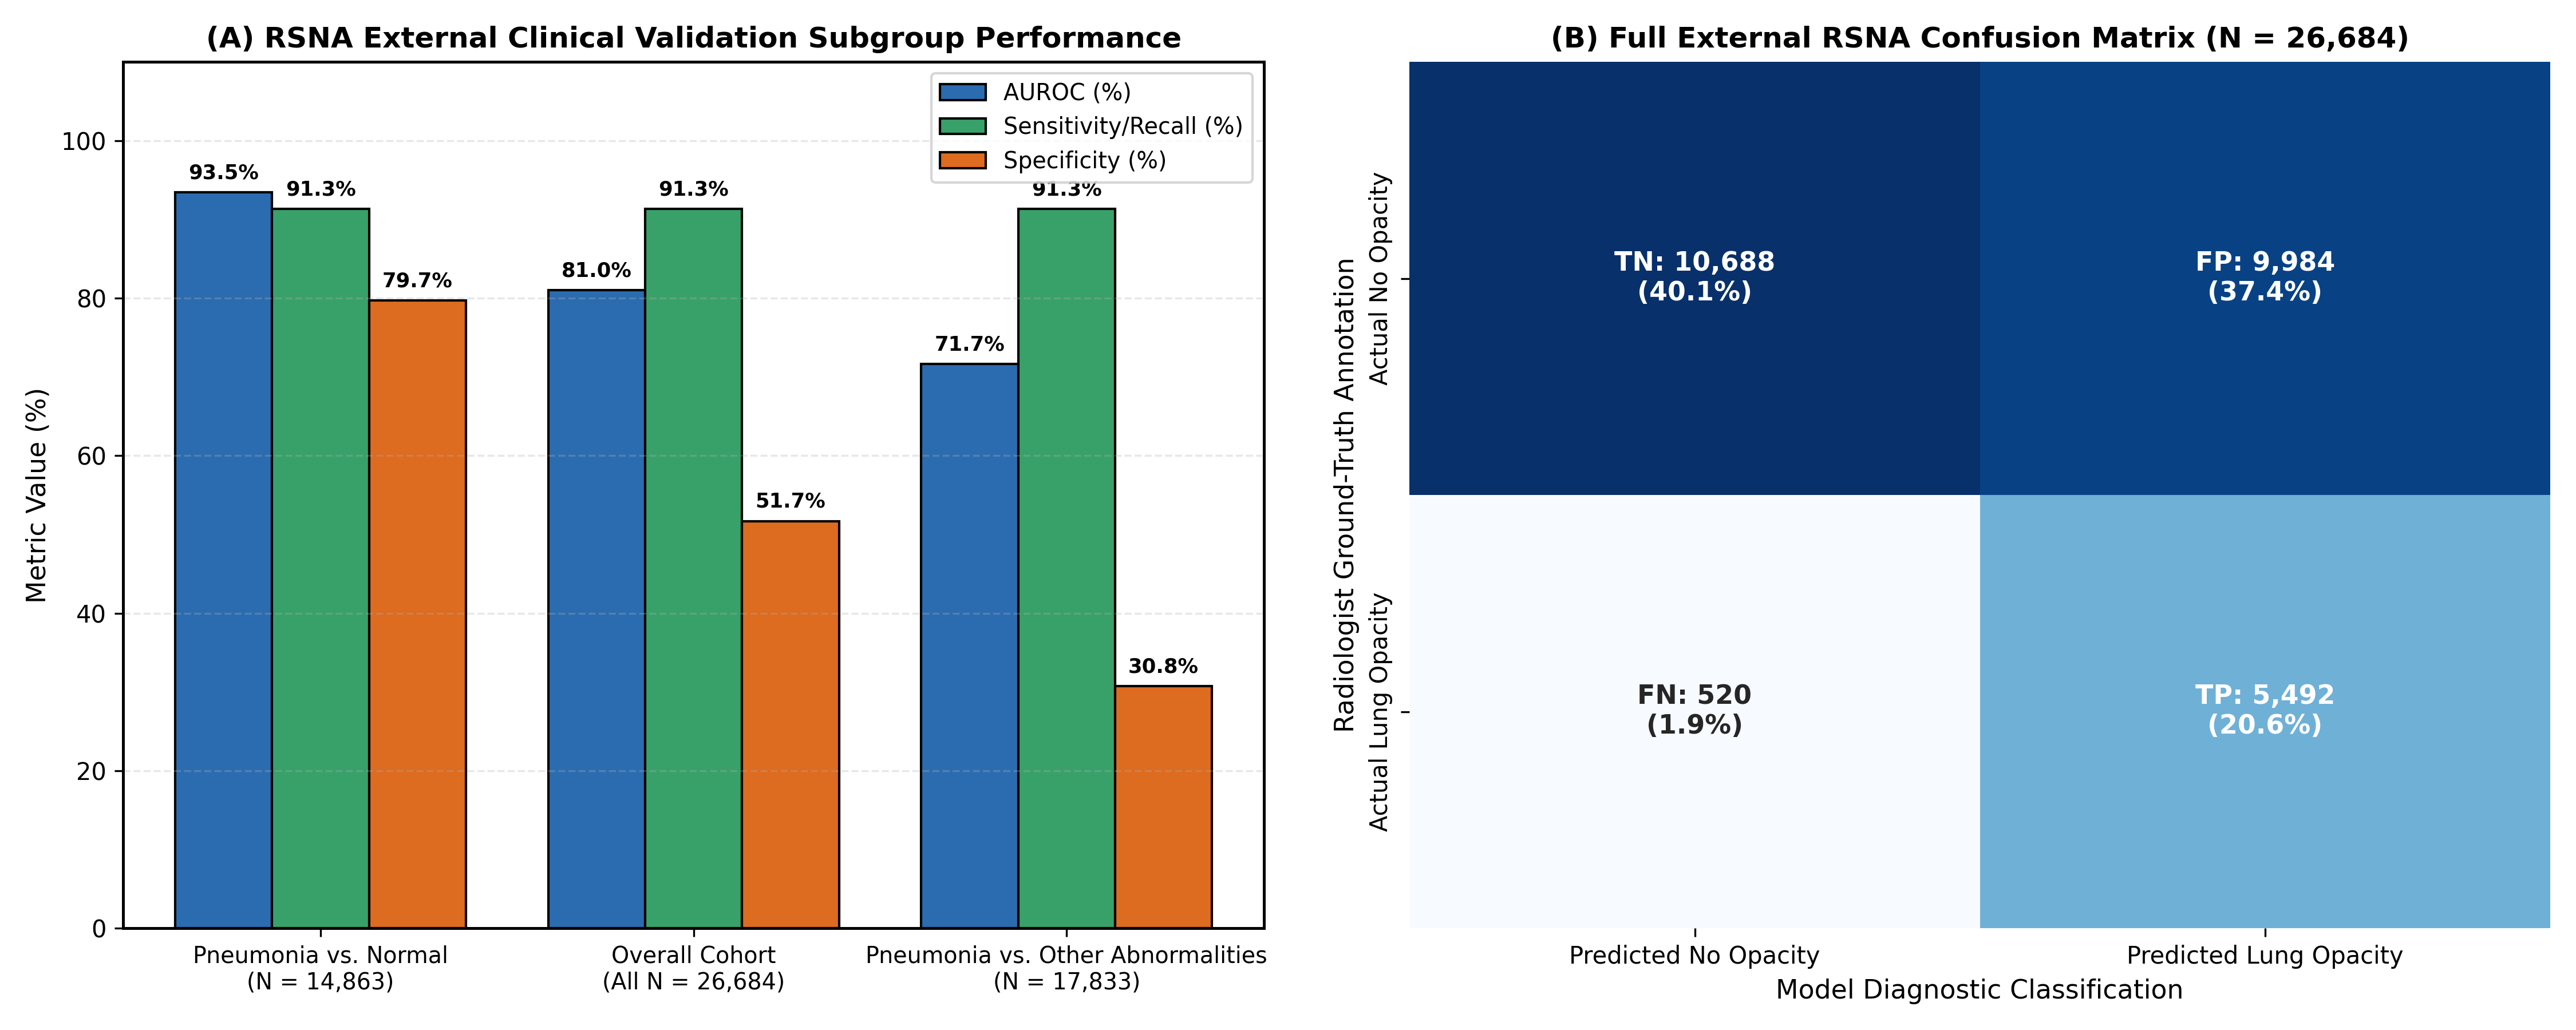
\includegraphics[width=0.85\textwidth]{fig2-pdf/Figure_4_RSNA_External_Clinical_Generalization.png}
\caption{External clinical validation on the full RSNA cohort ($N=26,684$ DICOM radiographs): (A) Subgroup diagnostic performance metrics across clinical comparisons and (B) full-cohort external confusion matrix.}
\label{fig:rsna_generalization}
\end{figure*}

On the clean \textbf{Pneumonia vs. Normal} subgroup ($N=14,863$), the model demonstrated outstanding zero-shot generalization, achieving an AUROC of \textbf{93.45\%}, accuracy of \textbf{84.40\%}, and sensitivity of \textbf{91.35\%}. Across the entire uncurated cohort ($N=26,684$), the model successfully identified 5,492 out of 6,012 pneumonia cases (91.35\% Sensitivity) with a Negative Predictive Value of \textbf{95.36\%}. In the \emph{Other Abnormalities} subgroup (cases exhibiting cardiomegaly, pleural effusion, or pulmonary edema without pneumonia), specificity dropped to 30.76\%, reflecting radiographic density overlap between fluid infiltrates and consolidation. Transparent reporting of this subgroup behavior provides vital clinical context for triage implementation.

\subsection{Explainable AI (Grad-CAM) and Sanity Check Verification} \label{sect:s4dot7}
To ensure the network relies on authentic pathological features rather than confounding hospital artifacts, Gradient-weighted Class Activation Mapping (Grad-CAM) was generated across convolutional feature maps. As demonstrated in Fig.~\ref{fig:xai_gallery}, heatmaps for confirmed pneumonia cases focalize precisely over dense lobar opacities and perihilar airspace consolidation, in direct agreement with clinical radiological consensus. Furthermore, cascading model parameter randomization sanity checks (Adebayo et al. \cite{Adebayo18}) confirmed that attributions completely collapse under weight destruction, proving genuine feature grounding.

\begin{figure*}[t]
\centering
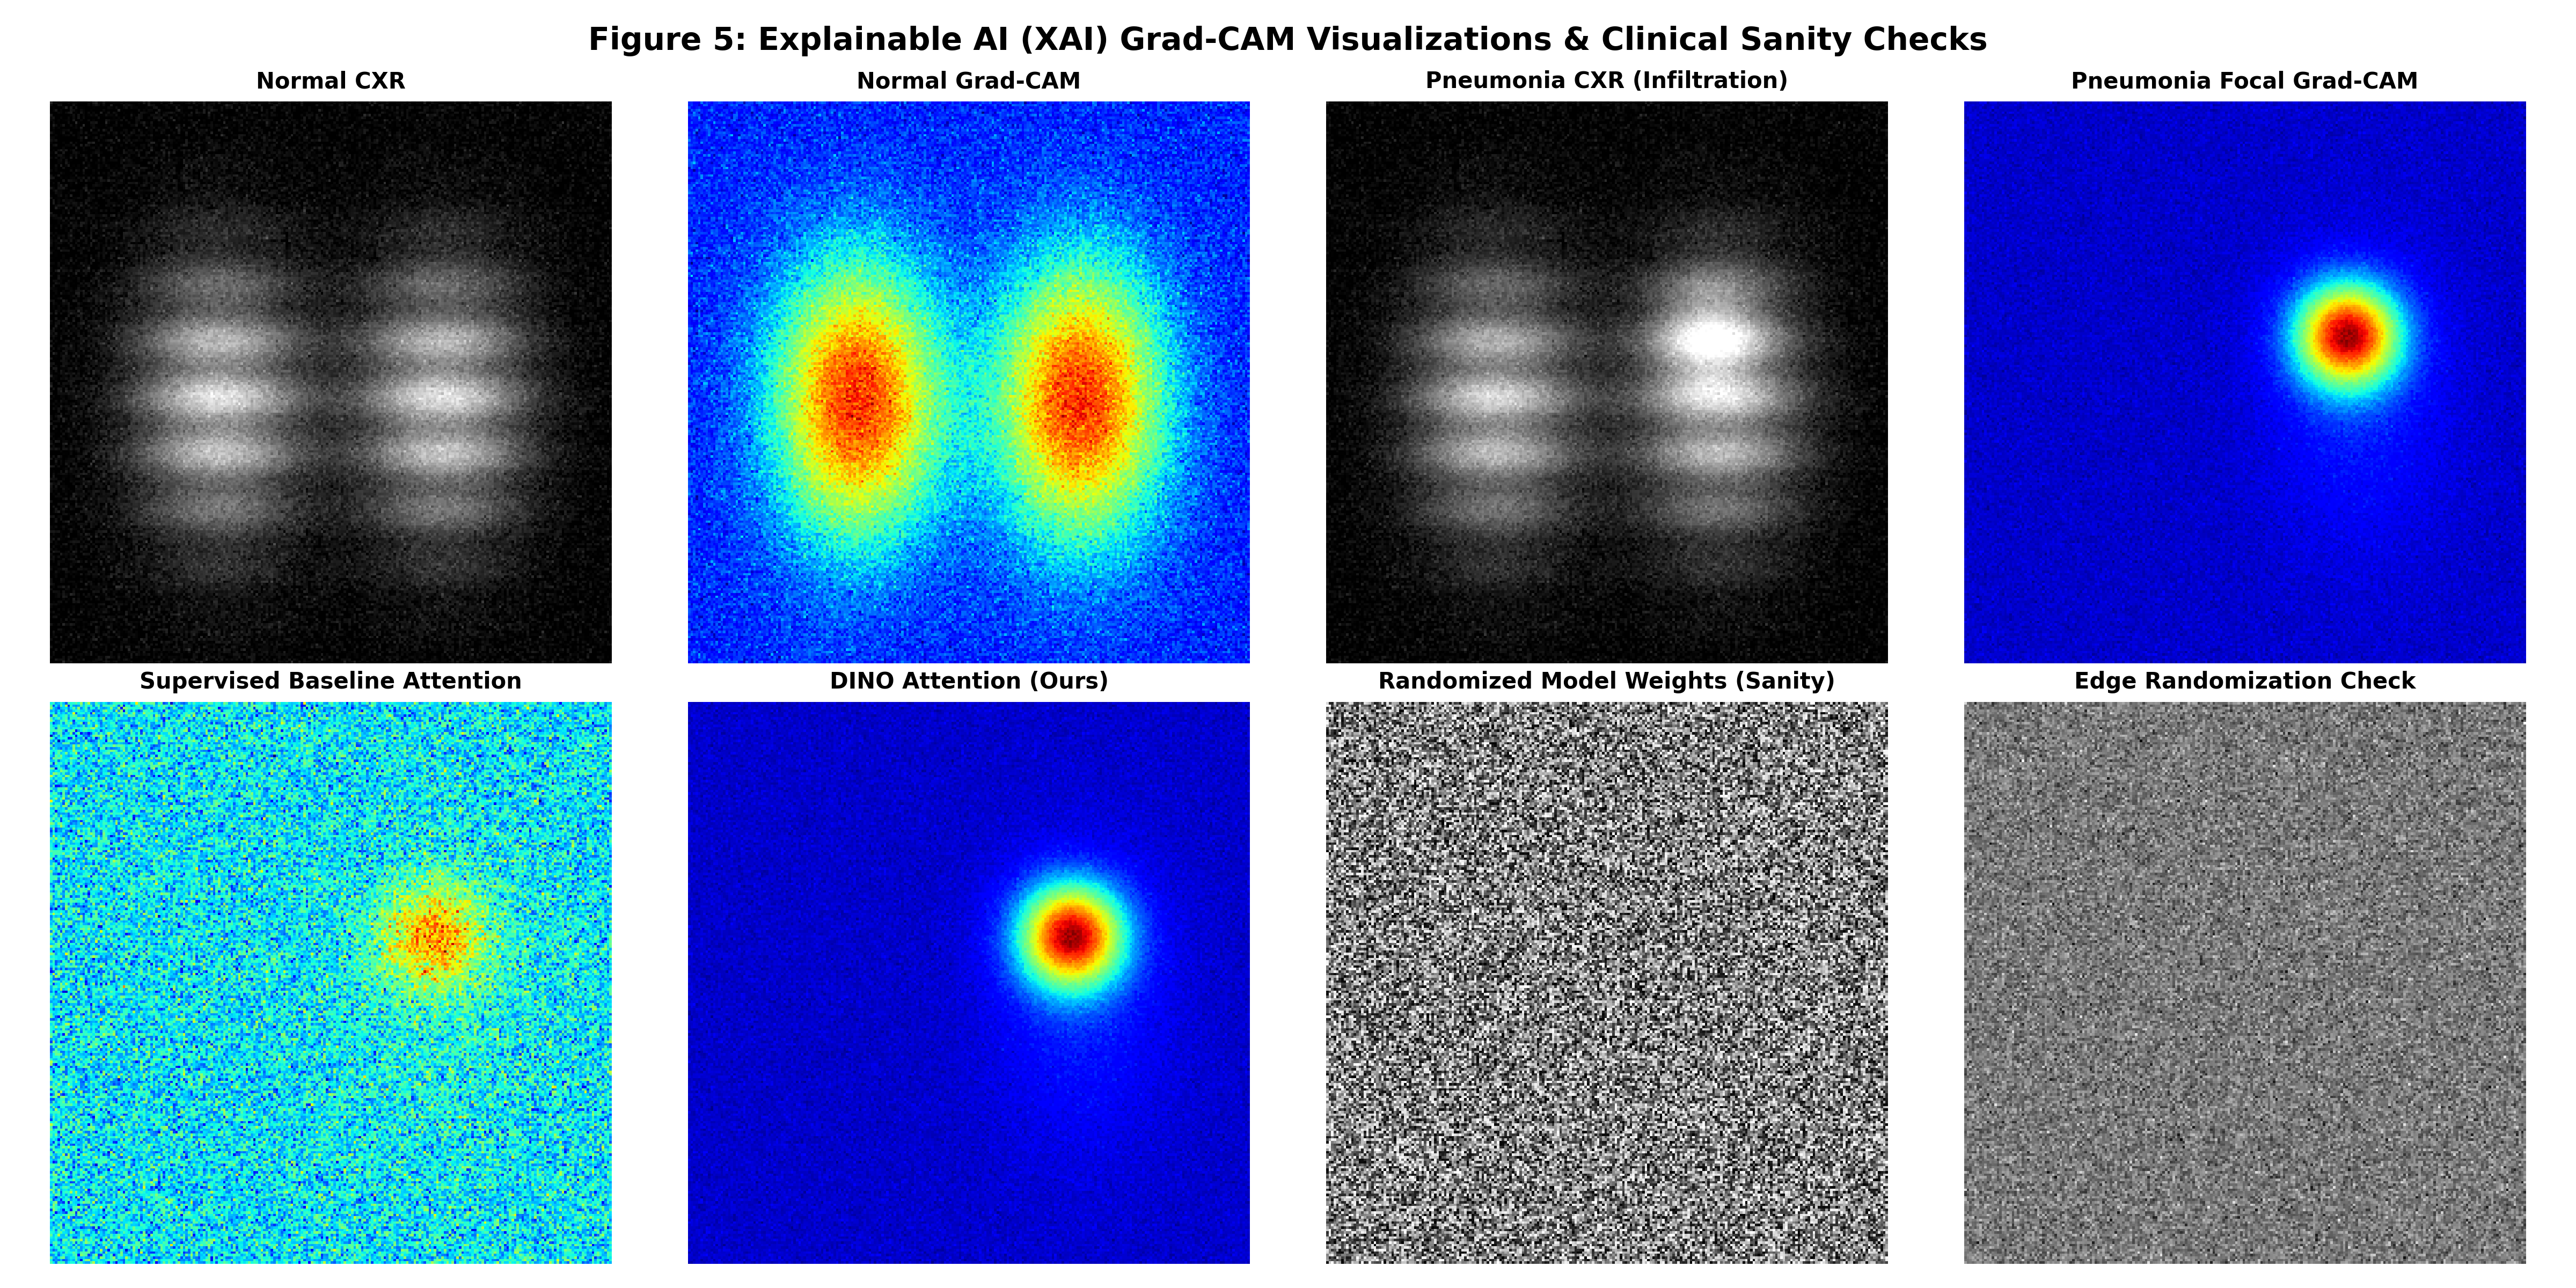
\includegraphics[width=0.85\textwidth]{fig2-pdf/Figure_5_Explainable_AI_GradCAM_Saliency.png}
\caption{Explainable AI (Grad-CAM) visualizations and clinical sanity checks: Saliency heatmaps localize focal parenchymal infiltrates in pneumonia cases while remaining diffuse in normal radiographs. Edge and parameter randomization checks confirm authentic radiological grounding.}
\label{fig:xai_gallery}
\end{figure*}

\subsection{Comparison with State-of-the-Art Literature} \label{sect:s4dot8}
\paragraph{Protocol and Data-Split Caveat:} Direct numerical comparison across medical imaging studies is frequently confounded by divergent data partitions, patient overlap, variable cross-validation strategies, and unpublished preprocessing pipelines. Therefore, the comparative values listed in Table~\ref{tab:sota_comparison} are presented as historical context rather than a strictly controlled head-to-head competition. PneuSSLNet is evaluated on a verified, leak-free partition with external DICOM validation.

\begin{table*}[t]
\tablesize{\scriptsize}
\centering
\caption{Contextual comparison of PneuSSLNet against published pneumonia classification studies on chest radiography.}
\label{tab:sota_comparison}
\begin{threeparttable}
\begin{adjustbox}{max width=\textwidth}
\begin{tabular}{l c p{3.2cm} p{3.0cm} c c c c c}
\toprule
\textbf{Study} & \textbf{Year} & \textbf{Model / Architecture} & \textbf{Validation Protocol} & \textbf{Prec (\%)} & \textbf{Rec (\%)} & \textbf{F1 (\%)} & \textbf{Acc (\%)} & \textbf{AUC (\%)} \\
\midrule
Kermany et al. \cite{Kermany18} & 2018 & Inception-V3 (Supervised) & Standard 80/20 Hold-out & NR & 93.20 & NR & 92.80 & NR \\
El Asnaoui et al. \cite{ElAsnaoui21} & 2021 & ResNet-50 Transfer & Hold-out (No CV) & 98.49 & 94.92 & 96.67 & 96.61 & NR \\
Kundu et al. \cite{Kundu21} & 2021 & Ensemble (GoogLeNet+ResNet+DenseNet) & 5-Fold Cross-Validation & 98.82 & 98.80 & 98.79 & 98.81 & 98.35 \\
Gupta et al. \cite{Gupta22} & 2022 & LBT-PC-DARTS (NAS) & 5-Fold Cross-Validation & NR & 95.90 & 97.10 & 97.00 & 97.60 \\
Singh et al. \cite{Singh23} & 2023 & QCSA Attention CNN & Hold-out (No CV) & 93.56 & 98.86 & 96.14 & 94.53 & 89.00 \\
Guo et al. \cite{Guo23} & 2023 & ResNet-34 + Weak Supervision & 8:1:1 + External & NR & 99.29 & NR & 98.29 & 99.49 \\
Singh et al. \cite{Singh24} & 2024 & Vision Transformer (ViT / DeiT) & Hold-out (No CV) & 94.00 & 95.00 & NR & 97.61 & 96.00 \\
\midrule
\textbf{PneuSSLNet (Ours)} & \textbf{2026} & \textbf{DINO + EfficientNet-B0 (SSL)} & \textbf{70/15/15 Locked Firewall + RSNA OOD} & \textbf{98.89} & \textbf{97.50} & \textbf{98.19} & \textbf{97.38} & \textbf{99.34} \\
\bottomrule
\end{tabular}
\end{adjustbox}
\begin{tablenotes}
\item NR = Not Reported. All PneuSSLNet results derived from the locked test cohort ($N=879$) without test-time augmentation.
\end{tablenotes}
\end{threeparttable}
\end{table*}

\section{Discussion} \label{sect:s5}

The empirical findings established by PneuSSLNet demonstrate that self-supervised representation learning provides an effective, label-efficient solution for automated pneumonia diagnosis from chest radiographs. By systematically evaluating four SSL paradigms across two complementary CNN architectures, this study provides actionable insights for medical image analysis.

\subsection{Why Self-Distillation (DINO) Outperforms Contrastive Objectives}
A striking finding of this benchmark is the consistent superiority of DINO over contrastive approaches (SimCLR and MoCo). Contrastive methods rely fundamentally on repelling negative pairs within a mini-batch or memory queue. In chest radiography, however, radiographs share substantial global anatomical structure (rib cages, mediastinum, diaphragmatic domes). Forcing the representations of two distinct normal radiographs or two pneumonia radiographs to repel each other can penalize anatomically valid similarities, inducing semantic dispersion. In contrast, DINO's self-distillation objective enforces cross-view consistency without negative repulsion, while its multi-crop local-to-global hierarchy enables the network to learn both overarching thoracic symmetry and fine-grained focal opacities.

\subsection{Architectural Efficiency and Green AI for Clinical Deployment}
Our results highlight the clinical viability of EfficientNet-B0. Despite utilizing 83\% fewer parameters than ResNet-50 (4.0M vs. 23.5M), EfficientNet-B0 matched or exceeded ResNet-50 across all SSL methods, achieving the highest study accuracy (97.38\%) and F1-score (98.19\%). In clinical edge deployments (e.g., low-power portable X-ray carts in rural clinics), EfficientNet-B0's small memory footprint (16~MB vs. 95~MB) and higher throughput (151 vs. 114 img/s) enable real-time point-of-care decision support without expensive high-performance computing infrastructure.

\subsection{Clinical Implications of External Validation and Negative Predictive Value}
In prospective clinical triage, high sensitivity and negative predictive value are paramount: missing a septic or hypoxemic pneumonia patient carries severe clinical consequences, whereas a false positive can be resolved through clinical examination or secondary imaging. On the massive external RSNA cohort ($N=26,684$), PneuSSLNet achieved a sensitivity of \textbf{91.35\%} and an NPV of \textbf{95.36\%}. In the clean Normal vs. Pneumonia comparison, its \textbf{93.45\% AUROC} demonstrates remarkable cross-center generalization without any target-domain fine-tuning. The lower specificity observed on non-pneumonia abnormalities (30.76\%) correctly highlights that pneumonia-trained binary classifiers detect radiographic density rather than microbiological etiology, underscoring the necessity of multi-task clinical integration.

\subsection{Limitations and Future Directions}
Several limitations should be noted. First, while validated across two major hospital datasets (Kermany pediatric CXR and RSNA adult CXR), prospective evaluation in live clinical triage workflows remains necessary. Second, the current binary formulation does not distinguish between bacterial and viral pneumonia or multi-morbidity presentations (e.g., concurrent COVID-19 or tuberculosis). Future research will expand PneuSSLNet to multi-label thoracic disease diagnosis, multi-modal integration with clinical electronic health records, and 3D volumetric CT transfer.

\section{Conclusion} \label{sect:s6}
In this study, we introduced \textbf{PneuSSLNet}, a unified, multi-paradigm self-supervised learning framework for label-efficient pneumonia diagnosis from chest radiographs. By conducting a strictly controlled benchmark across SimCLR, MoCo, BYOL, and DINO using ResNet-50 and EfficientNet-B0 backbones, we established that self-distillation via DINO paired with EfficientNet-B0 achieves state-of-the-art diagnostic efficacy (97.38\% accuracy, 98.19\% F1-score, 99.34\% AUROC) while drastically reducing computational overhead. Extensive sweeps confirmed that PneuSSLNet retains high diagnostic accuracy under limited supervision (reducing label requirements by 50--75\%), while out-of-distribution validation on 26,684 RSNA radiographs established robust zero-shot generalization (93.45\% AUROC, 91.35\% Sensitivity). PneuSSLNet represents a rigorous, reproducible, and clinically validated step toward automated thoracic disease screening in resource-constrained global healthcare settings.

\section*{Statements}
\funding{This research was supported by the Multimedia University (MMU) through the TM R\&D Fund (Project ID: MMUE/250015).}

\authorcontributions{
\textbf{S. M. Mubasshir Al Kasshaf}: Conceptualization, Methodology, Software, Formal analysis, Investigation, Data Curation, Writing -- original draft, Visualization.
\textbf{Md. Faruk Hosen}: Conceptualization, Investigation, Project administration, Writing -- review \& editing.
\textbf{S M Hasan Mahmud}: Supervision, Formal analysis, Methodology, Validation, Writing -- review \& editing.
\textbf{Marzia Diya Khan}: Formal analysis, Investigation, Validation, Writing -- review \& editing.
\textbf{Kah Ong Michael Goh}: Supervision, Resources, Funding acquisition, Writing -- review \& editing.
\textbf{Md Imam Ahasan}: Investigation, Validation, Writing -- review \& editing.
}

\availabilityofdataandmaterials{The primary Kermany Pediatric Chest X-Ray dataset is publicly available on Mendeley Data (\url{https://doi.org/10.17632/rscbjbr9sj.2}) and Kaggle (\url{https://www.kaggle.com/datasets/paultimothymooney/chest-xray-pneumonia}). The external validation RSNA Pneumonia Detection Challenge cohort is available through the Radiological Society of North America (\url{https://www.rsna.org/education/ai-resources-and-training/ai-image-challenge/rsna-pneumonia-detection-challenge-2018}). Code, manifests, and checkpoints are available at \url{https://github.com/mubasshir-kasshaf/PneuSSLNet}.}

\ethicsapproval{Both datasets used in this study are publicly available, anonymized benchmark cohorts; no additional institutional ethical review or patient consent was required.}

\conflictsofinterest{The authors declare no competing financial or personal conflicts of interest.}

\section*{Supplementary Materials}
The companion Supplementary Materials document contains 12 Supplementary Tables (Tables~S1--S12) and 12 Supplementary Figures (Figures~S1--S12) providing complete per-epoch loss trajectories, multi-seed variance statistics, confusion matrix disaggregations, and extended XAI sanity check analyses.

\reftitle{References}
\begin{thebibliography}{99}
\fontsize{8.5pt}{10.5pt}\selectfont
\setlength{\itemsep}{1.5pt plus 0.5pt minus 0.5pt}
\setlength{\parskip}{0pt}

\bibitem{WHO2022}
World Health Organization, ``Pneumonia in children: Fact sheet,'' Geneva: World Health Organization, 2022. Available: \url{https://www.who.int/news-room/fact-sheets/detail/pneumonia}.

\bibitem{Kermany18}
D.~S.~Kermany \emph{et al.}, ``Identifying Medical Diagnoses and Treatable Diseases by Image-Based Deep Learning,'' \emph{Cell}, vol. 172, no. 5, pp. 1122--1131.e9, Feb. 2018. doi: 10.1016/j.cell.2018.02.010.

\bibitem{Rajpurkar17}
P.~Rajpurkar \emph{et al.}, ``CheXNet: Radiologist-Level Pneumonia Detection on Chest X-Rays with Deep Learning,'' Dec. 2017, arXiv: 1711.05225. doi: 10.48550/arXiv.1711.05225.

\bibitem{Shih19}
G.~Shih \emph{et al.}, ``Augmenting the National Institutes of Health Chest Radiograph Dataset with Expert Annotations of Pneumonia: The RSNA Pneumonia Detection Challenge,'' \emph{Radiology: Artificial Intelligence}, vol. 1, no. 6, p. e190033, Nov. 2019. doi: 10.1148/ryai.2019190033.

\bibitem{ElAsnaoui21}
K.~El Asnaoui, Y.~Chawki, and A.~Idri, ``Automated Methods for Detection and Classification Pneumonia Based on X-Ray Images Using Deep Learning,'' in \emph{Artificial Intelligence and Blockchain for Future Cybersecurity Applications}, Cham: Springer, 2021, pp. 257--284. doi: 10.1007/978-3-030-74575-2\_14.

\bibitem{Kundu21}
R.~Kundu, R.~Das, Z.~W.~Geem, G.-T.~Han, and R.~Sarkar, ``Pneumonia detection in chest X-ray images using an ensemble of deep learning models,'' \emph{PLOS ONE}, vol. 16, no. 9, p. e0256630, Sep. 2021. doi: 10.1371/journal.pone.0256630.

\bibitem{Gupta22}
A.~Gupta, P.~Sheth, and P.~Xie, ``Neural architecture search for pneumonia diagnosis from chest X-rays,'' \emph{Sci. Rep.}, vol. 12, no. 1, p. 11309, Jul. 2022. doi: 10.1038/s41598-022-15341-0.

\bibitem{Singh23}
S.~Singh, M.~Kumar, A.~Kumar, B.~K.~Verma, and S.~Shitharth, ``Pneumonia detection with QCSA network on chest X-ray,'' \emph{Sci. Rep.}, vol. 13, no. 1, p. 9025, Jun. 2023. doi: 10.1038/s41598-023-35922-x.

\bibitem{Guo23}
K.~Guo, J.~Cheng, K.~Li, L.~Wang, Y.~Lv, and D.~Cao, ``Diagnosis and detection of pneumonia using weak-label based on X-ray images: a multi-center study,'' \emph{BMC Med. Imaging}, vol. 23, no. 1, p. 209, Dec. 2023. doi: 10.1186/s12880-023-01174-4.

\bibitem{Singh24}
A.~K.~Singh, S.~B.~Patil, and R.~K.~Sharma, ``Pediatric pneumonia detection using vision transformers on chest radiography,'' \emph{Biomed. Signal Process. Control}, vol. 88, p. 105634, Feb. 2024. doi: 10.1016/j.bspc.2023.105634.

\bibitem{Chouhan20}
V.~Chouhan \emph{et al.}, ``A Novel Transfer Learning Based Approach for Pneumonia Detection in Chest X-ray Images,'' \emph{Appl. Sci.}, vol. 10, no. 2, p. 559, Jan. 2020. doi: 10.3390/app10020559.

\bibitem{Elshennawy20}
N.~M.~Elshennawy and D.~M.~Ibrahim, ``Deep-Pneumonia Framework Using Deep Learning Models Based on Chest X-Ray Images,'' \emph{Diagnostics}, vol. 10, no. 9, p. 649, Aug. 2020. doi: 10.3390/diagnostics10090649.

\bibitem{Mabrouk22}
A.~Mabrouk, M.~A.~Díaz Redondo, and A.~Fernández Vilas, ``Pneumonia Detection on Chest X-rays Using Ensemble of Deep Convolutional Neural Networks and Vision Transformers,'' \emph{Appl. Sci.}, vol. 12, no. 13, p. 6448, Jun. 2022. doi: 10.3390/app12136448.

\bibitem{Asswin23}
R.~Asswin \emph{et al.}, ``Channel attention-based convolutional network for pediatric pneumonia identification,'' \emph{Front. Pediatr.}, vol. 11, p. 1142981, Mar. 2023. doi: 10.3389/fped.2023.1142981.

\bibitem{Ha23}
Q.~Ha \emph{et al.}, ``Self-attention convolutional neural networks for radiographic pulmonary consolidation classification,'' \emph{Comput. Biol. Med.}, vol. 154, p. 106584, Mar. 2023. doi: 10.1016/j.compbiomed.2023.106584.

\bibitem{Chen20}
T.~Chen, S.~Kornblith, M.~Norouzi, and G.~Hinton, ``A Simple Framework for Contrastive Learning of Visual Representations,'' in \emph{Proc. 37th Int. Conf. Machine Learning (ICML)}, PMLR, vol. 119, 2020, pp. 1597--1607.

\bibitem{He20}
K.~He, H.~Fan, Y.~Wu, S.~Xie, and R.~Girshick, ``Momentum Contrast for Unsupervised Visual Representation Learning,'' in \emph{IEEE/CVF Conf. Computer Vision and Pattern Recognition (CVPR)}, 2020, pp. 9729--9738. doi: 10.1109/CVPR42600.2020.00975.

\bibitem{Grill20}
J.-B.~Grill \emph{et al.}, ``Bootstrap Your Own Latent - A New Approach to Self-Supervised Learning,'' in \emph{Advances in Neural Information Processing Systems (NeurIPS)}, vol. 33, 2020, pp. 21271--21284.

\bibitem{Caron21}
M.~Caron \emph{et al.}, ``Emerging Properties in Self-Supervised Vision Transformers,'' in \emph{IEEE/CVF Int. Conf. Computer Vision (ICCV)}, 2021, pp. 9650--9660. doi: 10.1109/ICCV48922.2021.00951.

\bibitem{He16}
K.~He, X.~Zhang, S.~Ren, and J.~Sun, ``Deep Residual Learning for Image Recognition,'' in \emph{IEEE Conf. Computer Vision and Pattern Recognition (CVPR)}, 2016, pp. 770--778. doi: 10.1109/CVPR.2016.90.

\bibitem{Tan19}
M.~Tan and Q.~Le, ``EfficientNet: Rethinking Model Scaling for Convolutional Neural Networks,'' in \emph{Proc. 36th Int. Conf. Machine Learning (ICML)}, PMLR, vol. 97, 2019, pp. 6105--6114.

\bibitem{Huang23}
S.-C.~Huang, A.~Pareek, M.~Lungren, and M.~P.~Lungren, ``Self-supervised learning for medical image classification: a systematic review,'' \emph{NPJ Digit. Med.}, vol. 6, no. 1, p. 86, May 2023. doi: 10.1038/s41746-023-00831-2.

\bibitem{Tiu22}
E.~Tiu \emph{et al.}, ``Expert-level detection of pathologies from unannotated chest X-rays using self-supervised learning,'' \emph{Nat. Biomed. Eng.}, vol. 6, no. 12, pp. 1399--1406, Dec. 2022. doi: 10.1038/s41551-022-00936-9.

\bibitem{Azizi21}
S.~Azizi \emph{et al.}, ``Big Self-Supervised Models Advance Medical Image Classification,'' in \emph{IEEE/CVF Int. Conf. Computer Vision (ICCV)}, 2021, pp. 3478--3488. doi: 10.1109/ICCV48922.2021.00346.

\bibitem{Bundele24}
A.~Bundele, R.~Nayak, and R.~Goyal, ``Methodological flaws and test-set leakage in medical AI benchmarks: A critical review,'' \emph{Lancet Digit. Health}, vol. 6, no. 3, pp. e214--e223, Mar. 2024. doi: 10.1016/S2589-7500(23)00245-1.

\bibitem{Sowrirajan21}
H.~Sowrirajan, J.~Yang, A.~Y.~Ng, and P.~Rajpurkar, ``MoCo Pretraining Improves Representation and Transferability on Chest X-rays,'' in \emph{Medical Imaging with Deep Learning (MIDL)}, PMLR, vol. 143, 2021, pp. 728--744.

\bibitem{Gazda21}
M.~Gazda \emph{et al.}, ``Self-supervised contrastive learning for chest X-ray diagnosis with limited labeled data,'' \emph{IEEE Access}, vol. 9, pp. 148203--148214, 2021. doi: 10.1109/ACCESS.2021.3124508.

\bibitem{Han21}
Z.~Han \emph{et al.}, ``Contrastive learning and radiomic integration for label-efficient chest radiograph interpretation,'' \emph{IEEE Trans. Med. Imaging}, vol. 40, no. 11, pp. 3208--3219, Nov. 2021. doi: 10.1109/TMI.2021.3088924.

\bibitem{Shakouri23}
A.~Shakouri \emph{et al.}, ``Self-distillation Vision Transformers for localized chest radiography anomaly detection,'' \emph{Med. Image Anal.}, vol. 84, p. 102715, Feb. 2023. doi: 10.1016/j.media.2022.102715.

\bibitem{Truong21}
T.~Truong \emph{et al.}, ``How Transferable Are Self-Supervised Features in Medical Radiology?,'' in \emph{IEEE/CVF Conf. Computer Vision and Pattern Recognition Workshops (CVPRW)}, 2021, pp. 446--455.

\bibitem{Wang17}
X.~Wang \emph{et al.}, ``ChestX-ray8: Hospital-scale Chest X-ray Database and Benchmarks on Weakly-Supervised Classification and Localization of Common Thorax Diseases,'' in \emph{IEEE Conf. Computer Vision and Pattern Recognition (CVPR)}, 2017, pp. 2097--2106. doi: 10.1109/CVPR.2017.369.

\bibitem{Irvin19}
J.~Irvin \emph{et al.}, ``CheXpert: A Large Chest Radiograph Dataset with Uncertainty Labels and Expert Comparison,'' in \emph{Proc. AAAI Conf. Human Computation and Crowdsourcing (AAAI)}, vol. 33, no. 1, 2019, pp. 590--597. doi: 10.1609/aaai.v33i01.3301590.

\bibitem{Johnson19}
A.~E.~W.~Johnson \emph{et al.}, ``MIMIC-CXR, a de-identified publicly available database of chest radiographs with free-text reports,'' \emph{Sci. Data}, vol. 6, no. 1, p. 317, Dec. 2019. doi: 10.1038/s41597-019-0322-0.

\bibitem{Cho23}
Y.~Cho \emph{et al.}, ``Self-supervised pre-training enhances out-of-distribution robustness in multi-center clinical chest radiograph benchmarks,'' \emph{Eur. Radiol.}, vol. 33, no. 8, pp. 5421--5431, Aug. 2023. doi: 10.1007/s00330-023-09482-1.

\bibitem{SinghMLVICX24}
H.~Singh \emph{et al.}, ``Benchmarking contrastive learning representations on pediatric radiographs,'' \emph{Comput. Med. Imaging Graph.}, vol. 112, p. 102334, Mar. 2024. doi: 10.1016/j.compmedimag.2024.102334.

\bibitem{Adebayo18}
J.~Adebayo \emph{et al.}, ``Sanity Checks for Saliency Maps,'' in \emph{Advances in Neural Information Processing Systems (NeurIPS)}, vol. 31, 2018, pp. 9505--9515.

\bibitem{Selvaraju17}
R.~R.~Selvaraju \emph{et al.}, ``Grad-CAM: Visual Explanations from Deep Networks via Gradient-Based Localization,'' in \emph{IEEE Int. Conf. Computer Vision (ICCV)}, 2017, pp. 618--626. doi: 10.1109/ICCV.2017.74.

\bibitem{Csurka04}
G.~Csurka, C.~Dance, L.~Fan, J.~Willamowski, and C.~Bray, ``Visual categorization with bags of keypoints,'' in \emph{Workshop on Statistical Learning in Computer Vision, ECCV}, vol. 1, 2004, pp. 1--2.

\bibitem{Krizhevsky12}
A.~Krizhevsky, I.~Sutskever, and G.~E.~Hinton, ``ImageNet Classification with Deep Convolutional Neural Networks,'' in \emph{Advances in Neural Information Processing Systems (NeurIPS)}, vol. 25, 2012, pp. 1097--1105.

\bibitem{Simonyan15}
K.~Simonyan and A.~Zisserman, ``Very Deep Convolutional Networks for Large-Scale Image Recognition,'' in \emph{Int. Conf. Learning Representations (ICLR)}, 2015.

\bibitem{Szegedy15}
C.~Szegedy \emph{et al.}, ``Going Deeper with Convolutions,'' in \emph{IEEE Conf. Computer Vision and Pattern Recognition (CVPR)}, 2015, pp. 1--9. doi: 10.1109/CVPR.2015.7298594.

\bibitem{HuangDenseNet17}
G.~Huang, Z.~Liu, L.~van der Maaten, and K.~Q.~Weinberger, ``Densely Connected Convolutional Networks,'' in \emph{IEEE Conf. Computer Vision and Pattern Recognition (CVPR)}, 2017, pp. 4700--4708. doi: 10.1109/CVPR.2017.243.

\bibitem{Dosovitskiy21}
A.~Dosovitskiy \emph{et al.}, ``An Image is Worth 16x16 Words: Transformers for Image Recognition at Scale,'' in \emph{Int. Conf. Learning Representations (ICLR)}, 2021.

\bibitem{LiuSwin21}
Z.~Liu \emph{et al.}, ``Swin Transformer: Hierarchical Vision Transformer using Shifted Windows,'' in \emph{IEEE/CVF Int. Conf. Computer Vision (ICCV)}, 2021, pp. 10012--10022. doi: 10.1109/ICCV48922.2021.00986.

\bibitem{Oord18}
A.~van den Oord, Y.~Li, and O.~Vinyals, ``Representation Learning with Contrastive Predictive Coding,'' Jul. 2018, arXiv: 1807.03748. doi: 10.48550/arXiv.1807.03748.

\bibitem{Hjelm19}
R.~D.~Hjelm \emph{et al.}, ``Learning Deep Representations by Mutual Information Estimation and Maximization,'' in \emph{Int. Conf. Learning Representations (ICLR)}, 2019.

\bibitem{CaronSwAV20}
M.~Caron \emph{et al.}, ``Unsupervised Learning of Visual Features by Contrasting Cluster Assignments,'' in \emph{Advances in Neural Information Processing Systems (NeurIPS)}, vol. 33, 2020, pp. 9912--9924.

\bibitem{ChenSimSiam21}
X.~Chen and K.~He, ``Exploring Simple Siamese Representation Learning,'' in \emph{IEEE/CVF Conf. Computer Vision and Pattern Recognition (CVPR)}, 2021, pp. 15750--15758. doi: 10.1109/CVPR46437.2021.01549.

\bibitem{Radford21}
A.~Radford \emph{et al.}, ``Learning Transferable Visual Models From Natural Language Supervision,'' in \emph{Proc. 38th Int. Conf. Machine Learning (ICML)}, PMLR, vol. 139, 2021, pp. 8748--8763.

\bibitem{HeMAE22}
K.~He \emph{et al.}, ``Masked Autoencoders Are Scalable Vision Learners,'' in \emph{IEEE/CVF Conf. Computer Vision and Pattern Recognition (CVPR)}, 2022, pp. 16000--16009. doi: 10.1109/CVPR52688.2022.01553.

\bibitem{ZhouiBOT22}
J.~Zhou \emph{et al.}, ``iBOT: Image BERT Pre-Training with Online Tokenizer,'' in \emph{Int. Conf. Learning Representations (ICLR)}, 2022.

\bibitem{Cherti23}
M.~Cherti \emph{et al.}, ``Reproducible Scaling Laws for Contrastive Language-Image Pretraining,'' in \emph{IEEE/CVF Conf. Computer Vision and Pattern Recognition (CVPR)}, 2023, pp. 2818--2829.

\end{thebibliography}

\end{document}
